\newpage

\section{About me}\label{about-me}

I am a MSc student in Mathematical Modelling and Computation at DTU
(Technical University of Denmark). My main topic of interest of machine
learning, deep learning and artificial intelligence, as it applies to a
broad field of applications. This field field is about teaching machines
to identify patterns in data in order to perform tasks that have been
very difficult for machines traditionally.

\subsection{Motivation \& Area of
Interest}\label{motivation-area-of-interest}

About a 1.5 years ago I developed an interest in how humans learn,
learning efficiency and especially techniques for enhancing long-term
retention. This came out of a frustrating realization that I only
remember a small fraction of what I learned on my Bachelor degree in
Physics and Nanotechnology. It turns out that using spaced repetition,
it's actually possible to remember a much higher fraction of learned
material with relatively small effort - at least in theory. This is
possible due to the method of \emph{spaced practice}, where the average
time between recall sessions of information increases faster than
linearly. Intrigued by this possiblity, I experimented with using
\href{https://apps.ankiweb.net}{Anki}, a spaced repetition software
(SRS) in the fall semester of 2016. Ultimately I found it too time
consuming and I had other problems with it (which I will detail later),
so I dropped it mid-semester. I still thought it was a fundamentally
good idea that just needed better implementation of flashcard
organization, user interface and ease / speed of use.

I took the course ``Learning Technology and Digital Entrepreneurship''
to get inspiration for this spaced repetition software idea and to get
an introduction to various learning theories. It would also give me the
opportunity to read up on the latest on mathematical models of human
memory and spaced repetition.

After my first very rough prototype I developed during the course (see
Appendix \ref{sec:prototype}) I realized that the software platform I
envision should also have a strong collaborative component to allow
feedback and inspiration on flashcard decks. However, I was not prepared
for depth of the rabbit hole of spaced repetition research I was about
to enter. As it turns out, this is an area where extensive research has
been done for more than 100 years, and the number of citations on the
seminal paper that more or less started the field of memory research,
has been growing exponentially since the early 1980s
(Fig.~\ref{fig:ebbinghaus-citations}. It also turns out that the study
findings and recommendations coming out of study technique and memory
has largely been ignored. I dove deeply into the research literature
because I wanted to know what we know, and what we don't know. On that
basis I would then make an honest assessment about spaced repetition and
using flashcards. Due to my own failure of making it work, I was
prepared for the reality of the evidence perhaps not supporting the
efficiency of flashcards. That turned out not to be the case, and I'm
still very optimistic about the potential of this project.

\begin{figure}
\centering
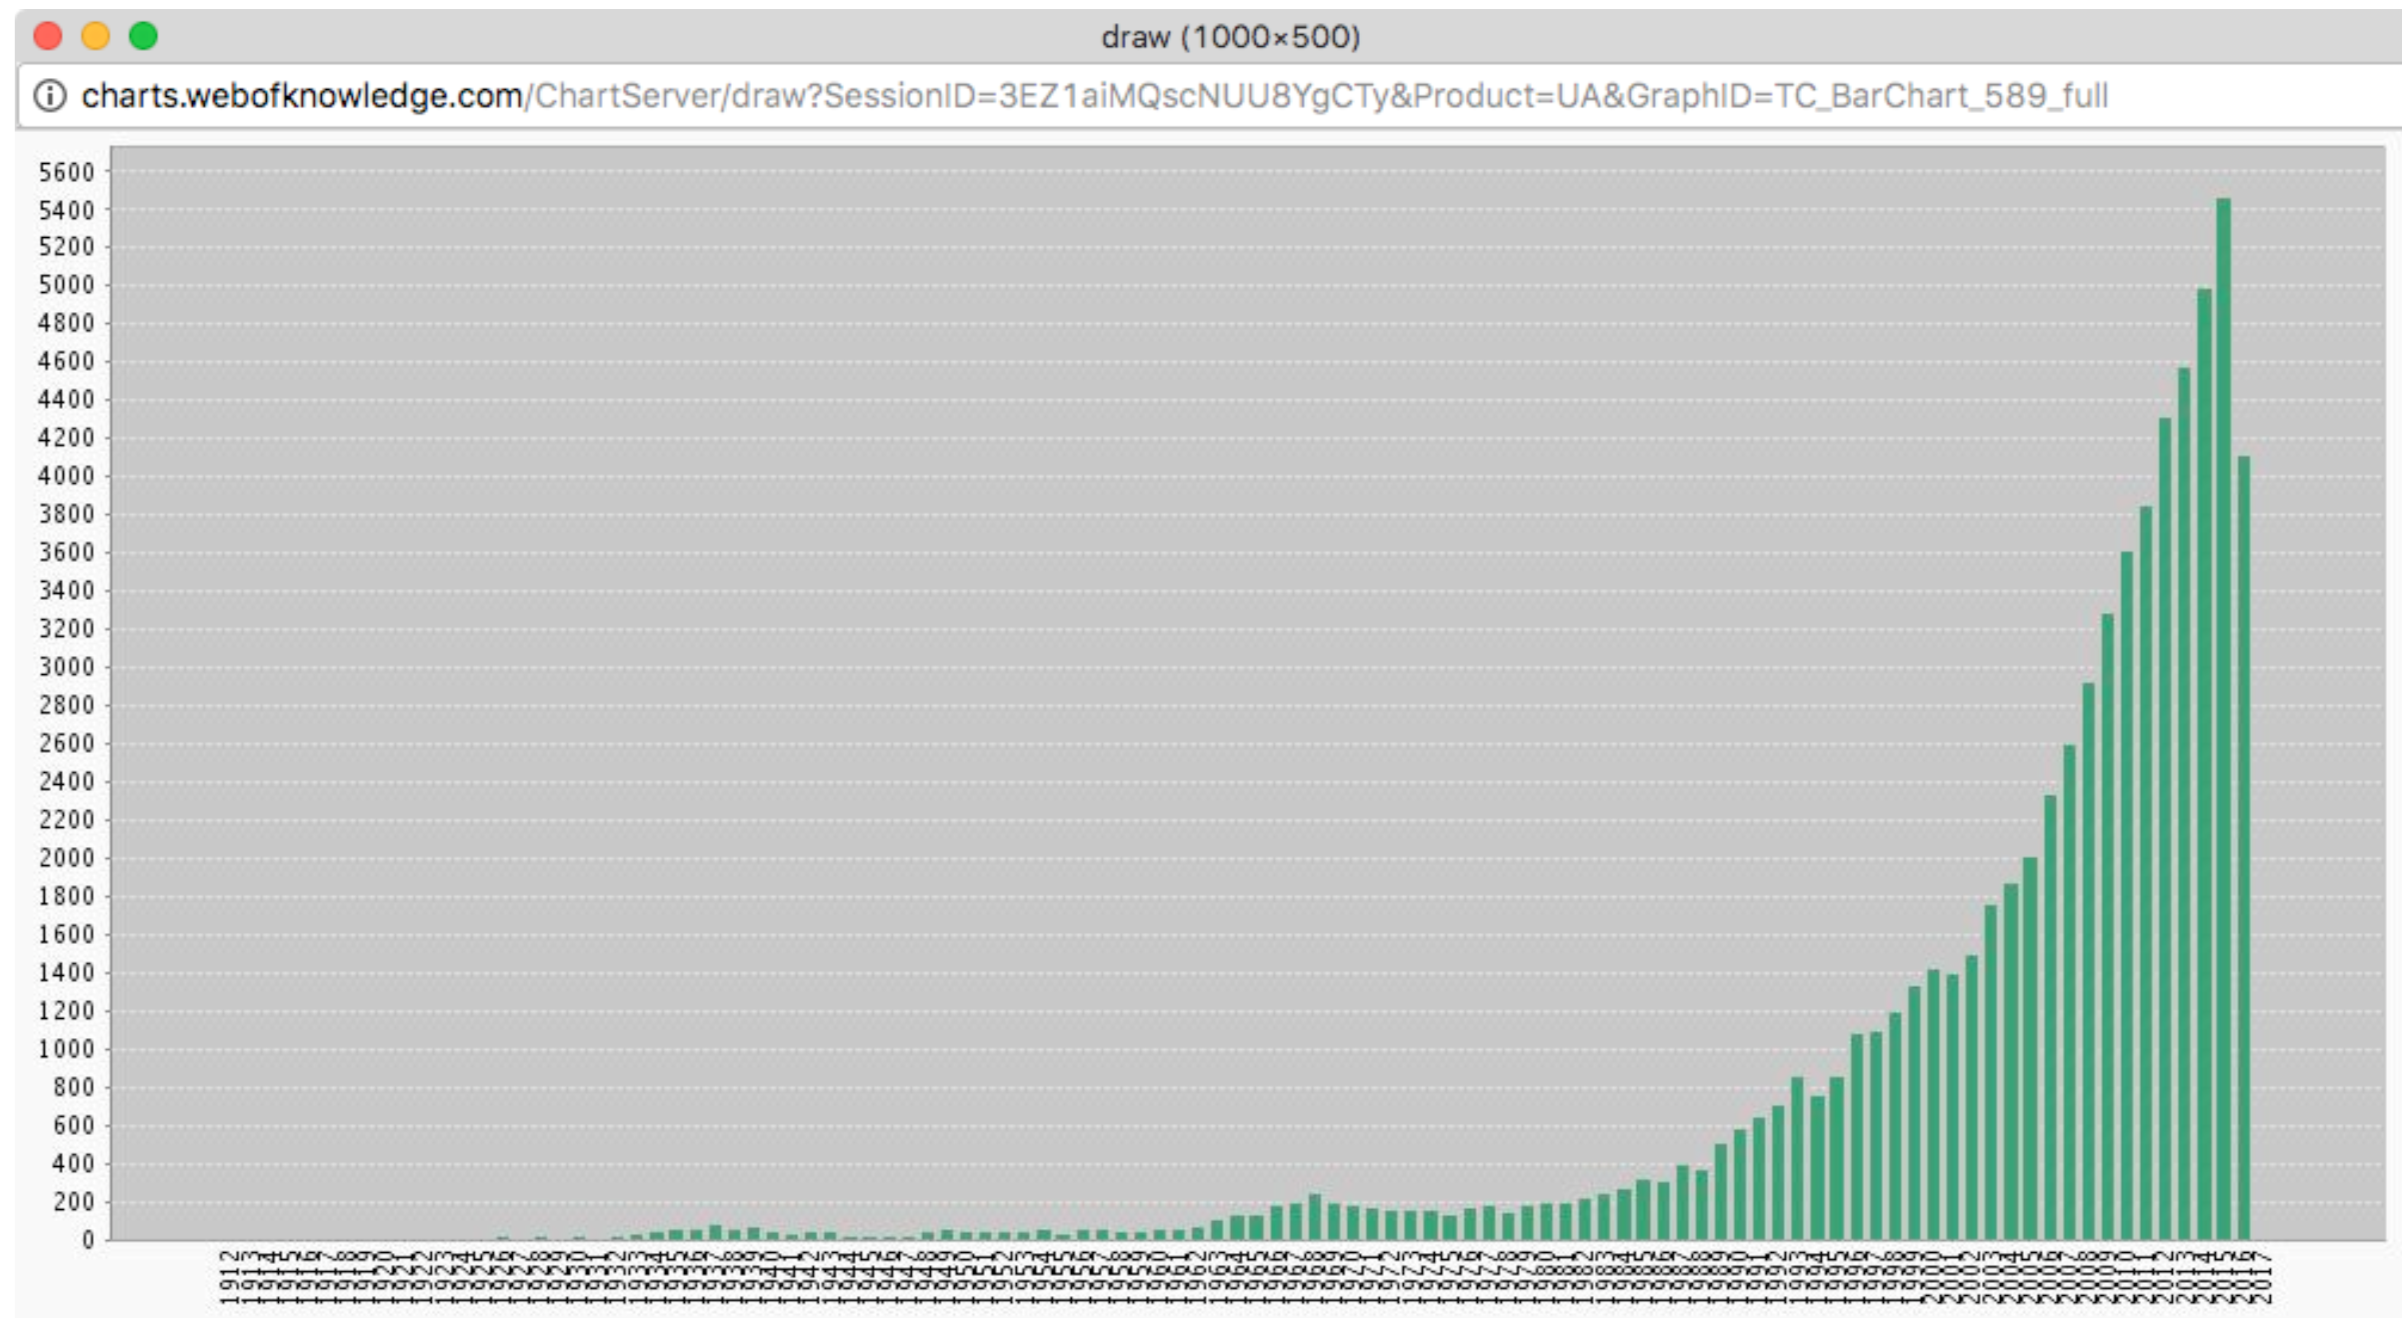
\includegraphics{assets/ebbinghaus-citations.png}
\caption{Citations of Hermann Ebbinghaus' 1885 paper years 1912---2016
(Subirana, Bagiati, and Sarma 2017). His work will be introduced in the
section on ``\protect\hyperlink{the-forgetting-curve}{The Forgetting
Curve}''}\label{fig:ebbinghaus-citations}
\end{figure}

\newpage

\section{Introduction}\label{introduction}

There are many examples of human traits that makes sense from our the
evolutionary path of our species, but that does not serve us so well
modern society. One of them may be how we use our memory. As (Subirana,
Bagiati, and Sarma 2017) noted:

\begin{quote}
From an evolutionary point of view, images and faces may be among the
oldest memory retention tasks for survival reasons (to recognize
friendly encounters and avoid invading dangerous settings or old
enemies).
\end{quote}

Our brains were never wired to remember vast amounts of mathematical
concepts, physical formulae, dynamics of economy, statistical analyses,
languages, and facts of many kinds. But perhaps we can take advantage of
what we do know about the memory to optimize retention.

Bryan Caplan is an economics professor at George Mason University and
interviewed in a piece for the 2018 January/February issue of The
Atlantic\footnote{https://www.theatlantic.com/magazine/archive/2018/01/whats-college-good-for/546590/},
said:

\begin{quote}
The conventional view---that education pays because students
learn---assumes that the typical student acquires, and retains, a lot of
knowledge. She doesn't. Teachers often lament summer learning loss:
Students know less at the end of summer than they did at the beginning.
But summer learning loss is only a special case of the problem of
fade-out: Human beings have trouble retaining knowledge they rarely use.
Of course, some college graduates use what they've learned and thus hold
on to it---engineers and other quantitative types, for example, retain a
lot of math. But when we measure what the average college graduate
recalls years later, the results are discouraging, to say the least.
\end{quote}

It seems plausible that engineers could be in a better position to
retain more of their studies than students of the humanities, depending
on how rigorously that learned material is applied. But there is still a
lot of room for improvement.

The paper ``On the Forgetting of College Academics: At `Ebbinghaus
Speed'?'' coming out of MIT Office of Digital Learning in June 2017
(Subirana, Bagiati, and Sarma 2017) opened with the abstract:

\begin{quote}
How important are Undergraduate College Academics after graduation? How
much do we actually remember after we leave the college classroom, and
for how long? Taking a look at major University ranking methodologies
one can easily observe they consistently lack any objective measure of
what content knowledge and skills students retain from college education
in the long term. Is there any rigorous scholarly published evidence on
retention of long-term unused academic content knowledge? We have found
no such evidence based on a preliminary literature review. Furthermore,
findings in all research papers reviewed in this study were consistent
with the following assertion: the Ebbinghaus forgetting curve
{[}Ebbinghaus 1880-1885{]} is a fundamental law of human nature -- in
fact, of the whole animal kingdom and applies to memory of all types:
verbal, visual, abstract, social and autobiographical. This fundamental
law of nature, when examined within the context of academic learning
retention, manifests itself as an exponential curve halving memory
saliency about every two years (what we call ``Ebbinghaus Speed''). This
paper presents the research group's initial hypothesis and conjectures
for college level education programming and curriculum development,
suggestions for instructional design enhancing learning durability, as
well as future research directions.
\end{quote}

I agree with the authors that the lack of long-term studies of skill
retention from college education is somewhat mystifying. The little
evidence there is seem to suggest an exponential decay (or ``Ebbinghaus
Curve'') with a half-life of two years. They go on:

\begin{quote}
Google, the best company to work for according to Fortune, has reported
to the New York Times that transcripts ``don't predict anything'' so
they have stopped asking for them, unless you are a few years out of
school. As a result Google has been hiring an increasing number of
employees without postsecondary education degrees. Google's approach is
consistent with the notion that everything is forgotten as our review
shows.
\end{quote}

The authors also note that despite STEM being ideal for testing the null
hypothesis of unused college academics being forgotten at ``Ebbinghaus
speed'', because STEM subjects are:

\begin{enumerate}
\def\labelenumi{\arabic{enumi}.}
\tightlist
\item
  Never used after the final exam
\item
  Difficult to master
\item
  Arguably completely unrelated to innate abilities
\end{enumerate}

Unfortunately, the most frequently studied elements by far are those of
syllables, series of words, words in a foreign language, personal
experiences, number series, emotional memories and the like. ``The
number of studies that explored memory retention by studying STEM
related content appeared to be extremely few and leave many doors
unexplored''. But there are a few studies, such as one that concluded
``About 50\% of what is learned in a Mechanics freshman class is lost by
the senior year unless it is re-used, in which case performance may even
improve.'', which is more or less in line with a knowledge half-life of
two years.

\begin{center}\rule{0.5\linewidth}{\linethickness}\end{center}

The learning platform I envision would be generally applicable to any
topic and learning situation, however it is designed with the subjects
of STEM (Science, Technology, Engineering, and Mathematics) in mind. I
think that STEM subjects and (medicine) are some the most challenging to
design spaced repetition software for. I will go in depth with the
reason for this in the section
``\protect\hyperlink{challenges-for-spaced-repetition}{Challenges for
spaced repetition}'', but STEM subjects is mainly challenging in
flashcards due to the high degree of interrelatedness of concepts.

In this collaborative learning platform, students following the same
course or topic of interest could help each other by sharing key
insights and take-away points they have learned from lectures or from
the reading material, and discuss it with each other. Furthermore,
everyone would be saving a collection of these ``highlights'' of
material and be making flashcards\footnote{A flashcard is a chunk of
  information with a que or question to trigger active recall of the
  memory} for themselves, which they could then revise using spaced
repetition.\footnote{Spaced repetition is repeated quizzing/retrieval of
  information, presenting easily recalled information less often and
  less memorized information more often.} The students should also be
able to rate and copy each other's flashcard decks, as well as raise
issues and questions about them.

This should support both learning and understanding during the course,
and also help to memorize key material well before the exam, thus
lightening the study load immediately before the exam. It would also
help long-term retention of the material, enabling people to remember
much more of what they learned long after the course ends (3 months, 1
year, 5 years etc.). The YouTube video ``Simulation of SRS
vs.~Traditional Review'' (Fig.~\ref{fig:memory-cells}) is a
visualization of a simple simulation of using spaced repetition
vs.~other kinds of material review when trying to remember a collection
of information.

\begin{figure}
\centering
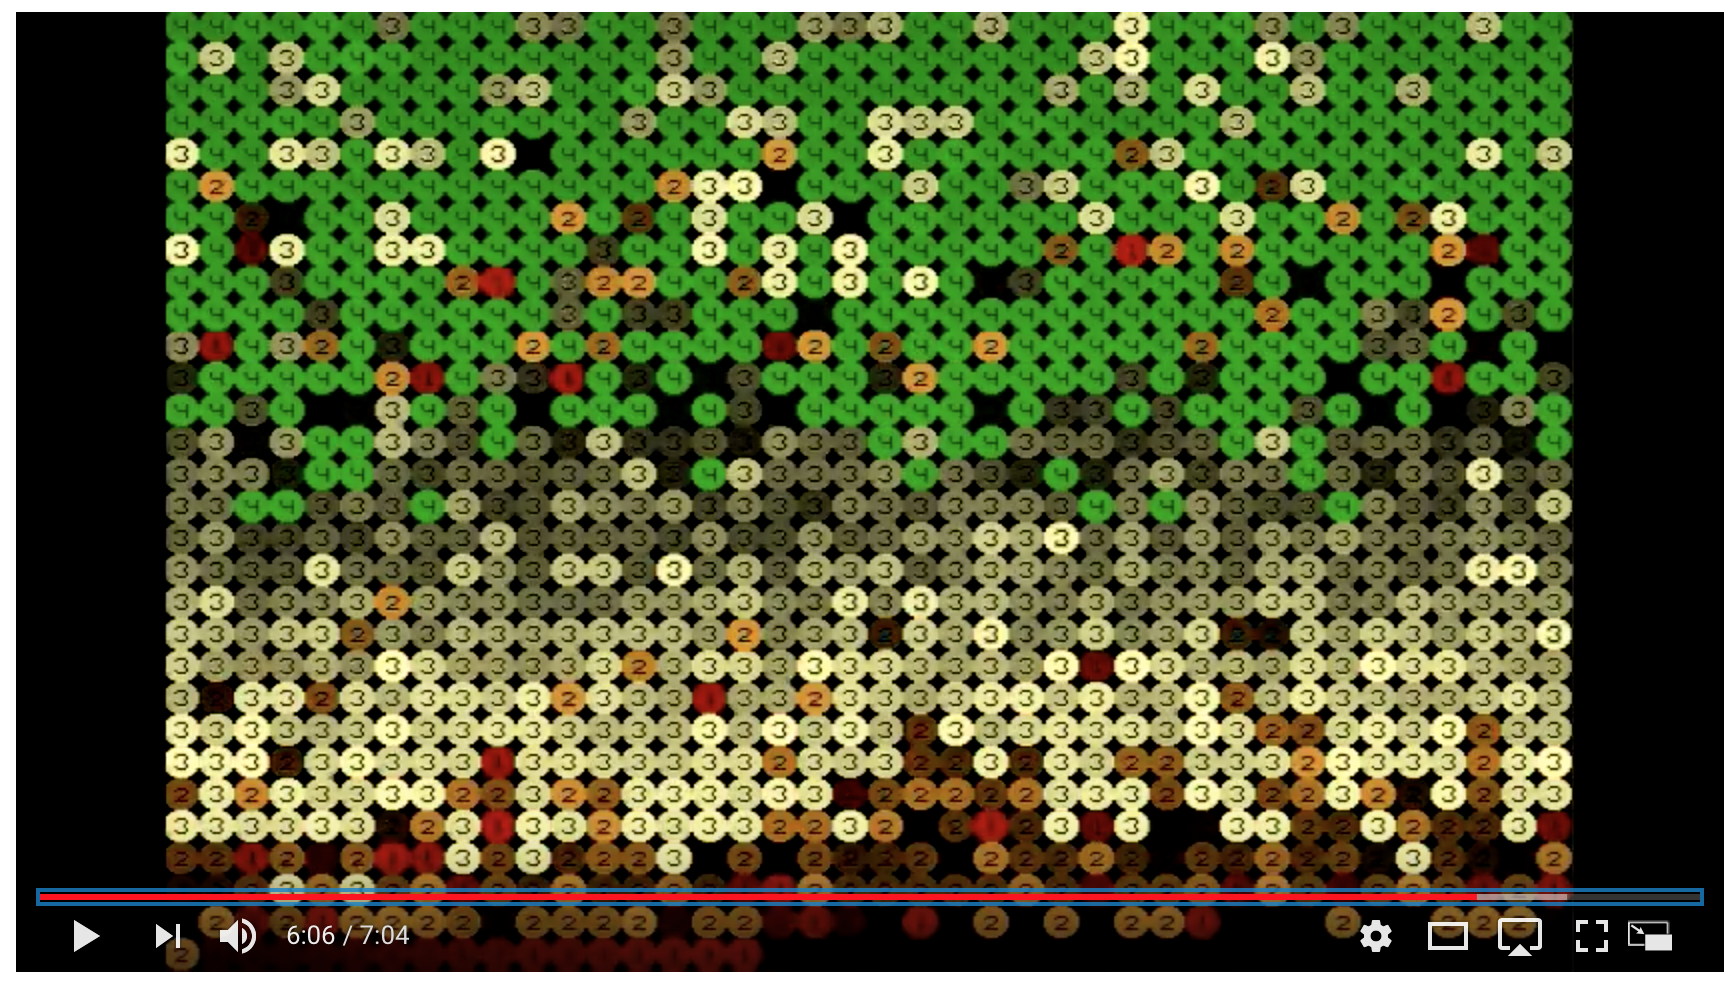
\includegraphics{assets/memory-cells.png}
\caption[The principle of spaced repetition visualized as memories being
energy cells that depletes with time at various rates. The video
showcases three different strategies for information review: 1. random,
2. recent and 3. spaced repetition. See video at.]{The principle of
spaced repetition visualized as memories being energy cells that
depletes with time at various rates. The video showcases three different
strategies for information review: 1. random, 2. recent and 3. spaced
repetition. See video at.\footnotemark{}}\label{fig:memory-cells}
\end{figure}
\footnotetext{https://www.youtube.com/watch?v=ai2K3qHpC7c}

(Kang 2016) notes (emphasis added by me):

\begin{quote}
Ample evidence supports the utility of spaced practice in improving
educational outcomes. Incorporating spaced practice into education can
be a cost-effective approach--- \textbf{learning becomes more durable in
the same amount of time (relative to massed practice), and this can lead
to future savings because less time needs to be spent on relearning
content that has been forgotten, leaving more time for other productive
learning activities} (e.g., higher order analysis, application of
knowledge). In short, spaced practice enhances the efficacy and
efficiency of learning, and it holds great promise as an educational
tool.
\end{quote}

\section{Problem Statement}\label{problem-statement}

The problem I wish to solve is two-fold:

\textbf{\#1 Much of what a student learns in a course or education is
forgotten soon after the exam.}

This is fine for the most part. We don't need \emph{all} the things we
learn during the course of our life and education. In fact, in a recent
article (Richards and Frankland 2017) published in the journal
\emph{Neuron}, neurobiologists Blake Richards and Paul Frankland
challenge the predominant view of memory, which holds that forgetting is
a process of loss (Terada 2017):

\begin{quote}
(\ldots{}) the goal of memory is not just to store information
accurately but to ``optimize decision-making'' in chaotic, quickly
changing environments. In this model of cognition, forgetting is an
evolutionary strategy, a purposeful process that runs in the background
of memory, evaluating and discarding information that doesn't promote
the survival of the species.

``From this perspective, forgetting is not necessarily a failure of
memory,'' explain Richards and Frankland in the study. ``Rather, it may
represent an investment in a more optimal mnemonic strategy.''
\end{quote}

One could even take the position that important core ideas will come up
more often in the course of education and work life, and therefore you
will naturally remember these recurrent subjects better than others, and
the whole thing works out as a self-optimizing system without the need
for a formal memory repetition system. I believe this is only half-true.

When one experience ``eureka moments'', some of these profound
experiences of deep understanding can leave such a lasting impression,
that you never really forget them; the feeling of a puzzle piece falling
into place in such a way that a big leap in understanding is achieved,
e.g.~some mathematical structure. Other information is basically
``fluff'' and will be rightfully buried in memory, as it should be, soon
after exposure. However in between these two extremes, there exists a
class of insights that are reasonably hard earned (or not) and that are
useful to remember, but many times forgotten almost completely. It seems
like a waste, because the work required to remember it much better is
actually not so substantial due to the shape of the forgetting curve
with repeated review intervals (introduced in a later chapter).

It is obviously desirable if a student was able to actively recall the
essential parts of her learning and training. One of the benefits would
be that many concepts are readily available to be applied without the
need to review. An arguably bigger benefit of having essential knowledge
well-retained is that ideas can be combined creatively. You can't Google
what you don't remember that you know.

\textbf{\#2 During the learning process, students could benefit from
each other so much more, with the right tools}

During the learning process, all student could benefit from more easily
being able to exchange ideas, insights and flashcard material. This
could form the basis if their exam preparation, that could then be done
gradually instead of being an intensive cramming session at the very
end.

\begin{center}\rule{0.5\linewidth}{\linethickness}\end{center}

In order for me to know what to look for as viable solutions to this
two-fold problem statement, I looked to what the scientific research
tells us about study techniques.

\newpage

\section{Research Overview on Study
Techniques}\label{research-overview-on-study-techniques}

\hypertarget{what-works}{\subsection{What Works}\label{what-works}}

A study of more than 700 scientific articles on 10 commonly used study
techniques showed that \emph{self-testing} and \emph{distributed
practice} are among the most universally effective study techniques
(Dunlosky et al. 2013). They classified study techniques into three
categories:

\subsubsection{Top strategies}\label{top-strategies}

These two study techniques showed consistently good results across age
and topics.

\begin{enumerate}
\def\labelenumi{\arabic{enumi}.}
\tightlist
\item
  \textbf{Self-testing:} Testing oneself in the material by actively
  recalling it from memory, as opposed to merely re-reading it and
  recognizing the information.
\item
  \textbf{Distributed practice:} Spreading out the studying over time as
  opposed to cramming just before the exam.
\end{enumerate}

From my own observations and from talking to my fellow students, these
study techniques are rarely used consistently by students. This is
likely due to a lack of awareness of study technique research, but I
believe it's also a result of a lack of good tools. In a later chapter I
will go more into depth with the software that is already available, and
how my proposal is different.

\subsubsection{The Runner ups}\label{the-runner-ups}

These three study techniques showed good results in some circumstances
and/or still needs more study to determine their usefulness.

\begin{enumerate}
\def\labelenumi{\arabic{enumi}.}
\setcounter{enumi}{2}
\tightlist
\item
  \textbf{Elaborative interrogation:} Asking yourself ``Why?'',
  recursively like a children do; ``Why does it make sense
  that\ldots{}?'' or ``Why is this true?''
\item
  \textbf{Self-explanation:} Asking yourself ``What new information does
  this sentence provide'' and ``How does this relate to what I already
  know?'' to make connection with existing knowledge.
\item
  \textbf{Interleaved practice:} Mixing up study sessions to study
  across the learned material so far instead of linearly trying to
  master the concepts one after another.
\end{enumerate}

I did found some newer studies with showed convincingly good results for
interleaved practice in real-world classroom settings (more on this in
the chapter \protect\hyperlink{interleaved-practice}{Interleaved
Practice}).

Another study (Prince 2004) also put emphasis on \textbf{peer-to-peer
explanations}: ``the best available evidence suggests that faculty
should structure their courses to promote collaborative and cooperative
environments''.

\subsection{What Doesn't Work}\label{what-doesnt-work}

\begin{itemize}
\tightlist
\item
  \textbf{Underlining:} was shown to be ineffective ``regardless of text
  length and topic, whether it was aerodynamics, ancient Greek schools
  or Tanzania'' (Dunlosky et al. 2013). It is theorized that it may be
  that underlining draws attention to individual items rather than
  connections across items. It is concluded that highlighting and
  underlining can be useful in the binning of a journey, if the marked
  information is subsequently turned into flashcards or other forms of
  self-test (Dunlosky et al. 2013).
\item
  \textbf{Re-reading:} The effectiveness of re-reading varied across
  different types of content, but no benefits were shown beyond the
  second reading, and self-testing was most often shown to be more
  effective than re-reading (Dunlosky et al. 2013).
\end{itemize}

The software proposal in the report will combine the two top methods
(self-testing and distributed practice), as well as peer-to-peer
explanations and optionally interleaved practice.

\hypertarget{the-forgetting-curve}{\section{The Forgetting
Curve}\label{the-forgetting-curve}}

Before we can try to solve the first problem in the problem statement,
we first need to understand roughly how the memory works.

Robert Bjork\footnote{https://www.psych.ucla.edu/faculty/page/bjork},
the director of the UCLA Learning and Forgetting Lab, a distinguished
professor of psychology, and a ``massively renowned expert on packing
things in your brain in a way that keeps them from leaking out'', says
in an interview with Wired in 2012 (``Everything You Thought You Knew
About Learning Is Wrong'' 2012):

\begin{quote}
``Forget about forgetting,'' said Bjork. ``People tend to think that
learning is building up something in your memory and that forgetting is
losing the things you built. But in some respects the opposite is
true.''

See, once you learn something, you never actually forget it. Do you
remember your childhood best friend's phone number? No? Well, Bjork
showed that if you were reminded, you would retain it much more quickly
and strongly than if you were asked to memorize a fresh seven-digit
number. So this old phone number is not forgotten -- it lives somewhere
in you -- but recall can be a bit tricky. And while we count forgetting
as the sworn enemy of learning, in some ways that's wrong, too. The two
live in a kind of symbiosis in which forgetting actually aids recall.

``Because humans have unlimited storage capacity, having total recall
would be a mess,'' said Bjork. ``Imagine you remembered all the phone
numbers of all the houses you had ever lived in. When someone asks you
your current phone number, you would have to sort it from this long
list.'' Instead, we forget the old phone numbers, or at least bury them
far beneath the ease of recall we gift to our current number. What you
thought were sworn enemies are more like distant collaborators.
\end{quote}

In 1885 the German psychologist Hermann Ebbinghaus tried to memorize a
collection of nonsense syllables, and studied how well he could remember
these afterwards. He published his seminal work of what would become
known as the \emph{forgetting curve}: a curve that shows memory
rentention (probablity of recalling some information) vs.~time. These
results have been replicated many times, one of the latest in a 2015
study (Murre and Dros 2015), see Fig.~\ref{fig:forgetting-curve}. They
found that less than 50\% of the syllables were forgotten after 24
hours.

\begin{figure}
\centering
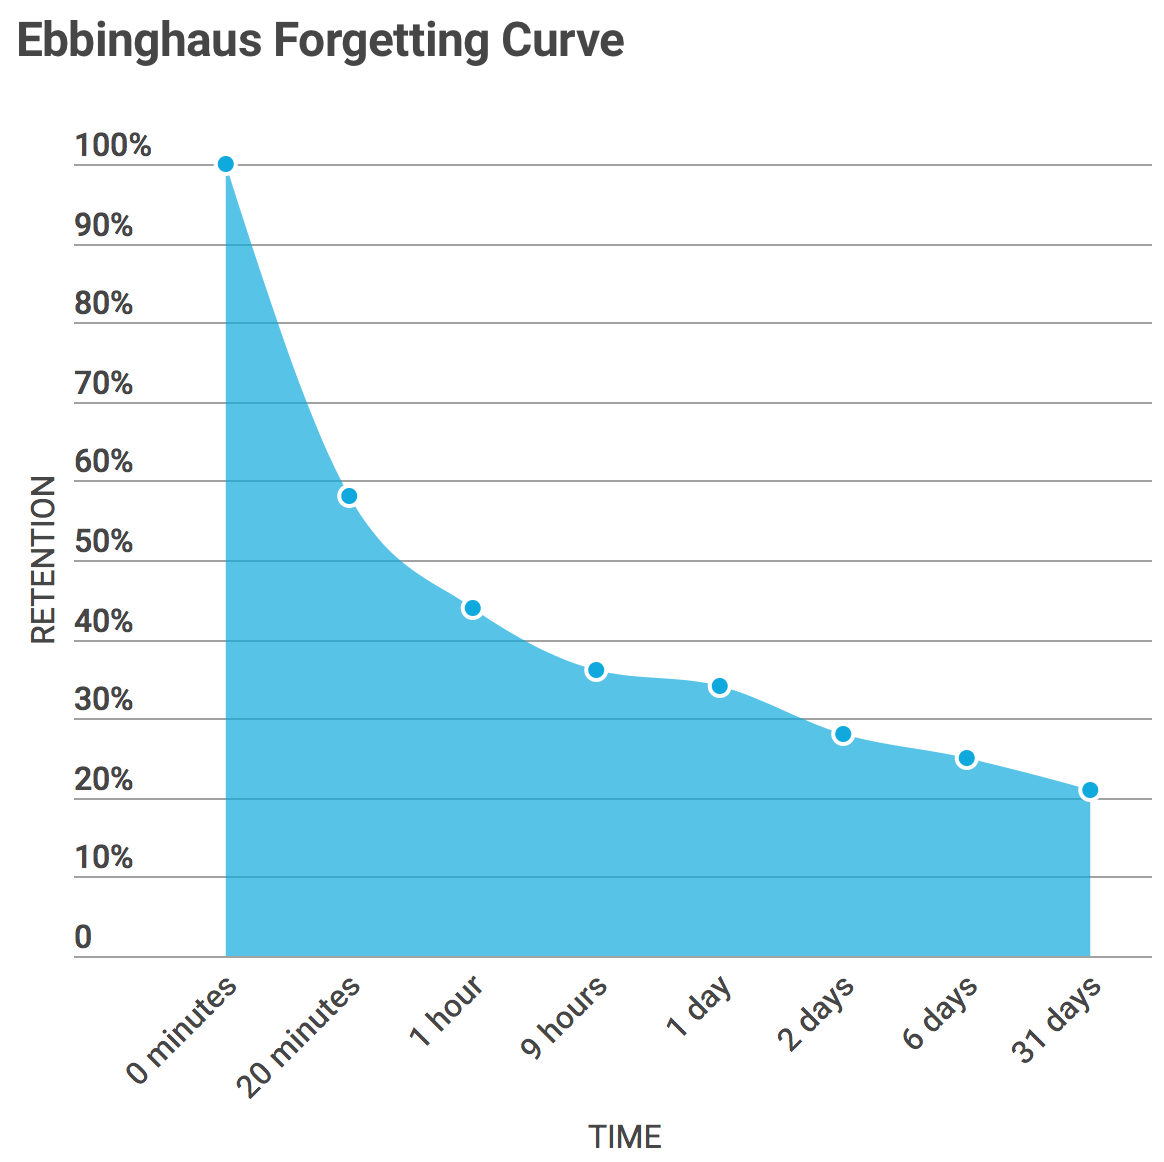
\includegraphics[width=0.65000\textwidth]{assets/ebbinghaus-forgetting-curive-2015.png}
\caption{Ebbinghaus forgetting curve replicated in (Murre and Dros
2015)}\label{fig:forgetting-curve}
\end{figure}

How about ``real'' course material instead of just nonsense syllables?
These typically show significantly longer lifetime, very likely because
meaningful information sticks easier to memory easier than nonsense
syllables. One study in 2006 that followed students of a consumer
behavior course (that included an introduction to statistics), concluded
that most of the knowledge gained was effectively lost within 2 years of
taking the course (Bacon and Stewart 2006), see
Fig.~\ref{fig:course-fcurve}.

\begin{figure}
\centering
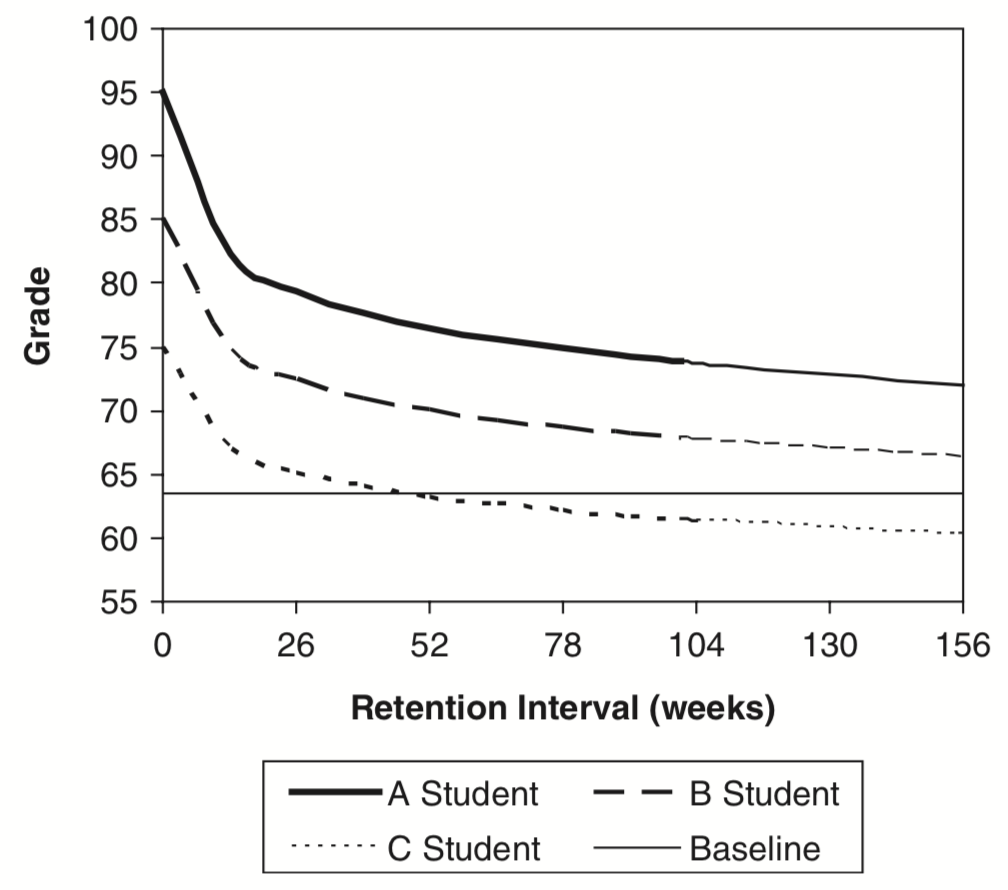
\includegraphics[width=0.60000\textwidth]{assets/forgetting-curve2.png}
\caption{Measured forgetting curve based on multiple choice test of 374
student in a consumer behavior course at a moderate-sized private
university in the Western United States, (Bacon and Stewart
2006)}\label{fig:course-fcurve}
\end{figure}

Another modern example of this loss of knowledge without repetition is a
study of cardiopulmonary resuscitation (CPR) skills that demonstrated
rapid decay in the year following training. By 3 years post-training
only 2.4\% were able to perform CPR successfully (Branwen 2009).

The exciting aspect of the forgetting curve is the shape of the curve
upon multiple reviews of the information. It turns out that the optimal
time intervals between successive reviews is, on average,
superlinear.\footnote{There has been some debate about uniformly spaced
  vs.~expanding review schedule, but the difference is not substantial,
  and the expanding schedule is more practical. More will be said on
  this later.} This in turn means progressively longer times between
needed review sessions of the particular information.

As an example, after having seen some information for the first time,
then in order to maintain a fixed threshold of probability to recall
this piece of information, review times could then be scheduled perhaps
24 hours, 1 day, 3 days, 7 days, 30 days, 6 months, 2 years etc., after
first encounter with the information, see Fig.~\ref{fig:sr} (sometimes
going a step back if the information is forgotten faster than expected).
In other words, it requires progressively less effort to keep things in
long-term memory. When done with multiple items, the result is that
things that are more easily remembered or seen less often, and things
that was harder to remember are seen more often, thus optimizing stidy
time. This technique is known as \emph{spaced repetition}.

\begin{figure}
\centering
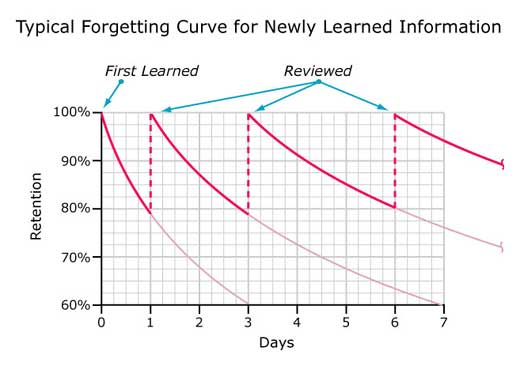
\includegraphics[width=0.75000\textwidth]{assets/spaced_repetition.jpg}
\caption[Spaced repetition is based on actively recalling information at
the optimal time, e.g.~at the time when there is 80\% chance of not
being able to recall it.]{Spaced repetition is based on actively
recalling information at the optimal time, e.g.~at the time when there
is 80\% chance of not being able to recall
it\footnotemark{}.}\label{fig:sr}
\end{figure}
\footnotetext{Source: http://www.ellaz.com/AIV/Strategy-3.aspx}

A study (Averell and Heathcote 2011) used maximum likelihood (ML)
analysis and Markov Chain Monte Carlo (MCMC) to estimate for parameter
estimation model selection (between exponential, power and pareto), for
a replication of the Ebbinghaus experiment. They found the power
function to be the best fit, although the difference between exponential
and power did not seem substantial.

We will look at newer models for human memory and scheduling in the
section
``\protect\hyperlink{optimal-spacing-schedule-for-spaced-repetition}{Optimal
Spacing Schedule for Spaced Repetition}''.

\subsubsection{The Leitner System}\label{the-leitner-system}

Scheduling these reviews individually could be a daunting task to do
manually. A simplified analog flashcard system was proposed by the
German science journalist Sebastian Leitner in the 1970s. There are a
number of boxes, for example 5, and all flashcards start in the first
box. All flashcards are practiced a number of times, and if answered
correctly then ``graduates'' to the next box, and if answered
incorrectly, either put in the previous box or reset to the first box. A
study schedule is then set such that boxes with higher numbers are
practiced less often than lower numbered boxes.

\begin{figure}
\centering
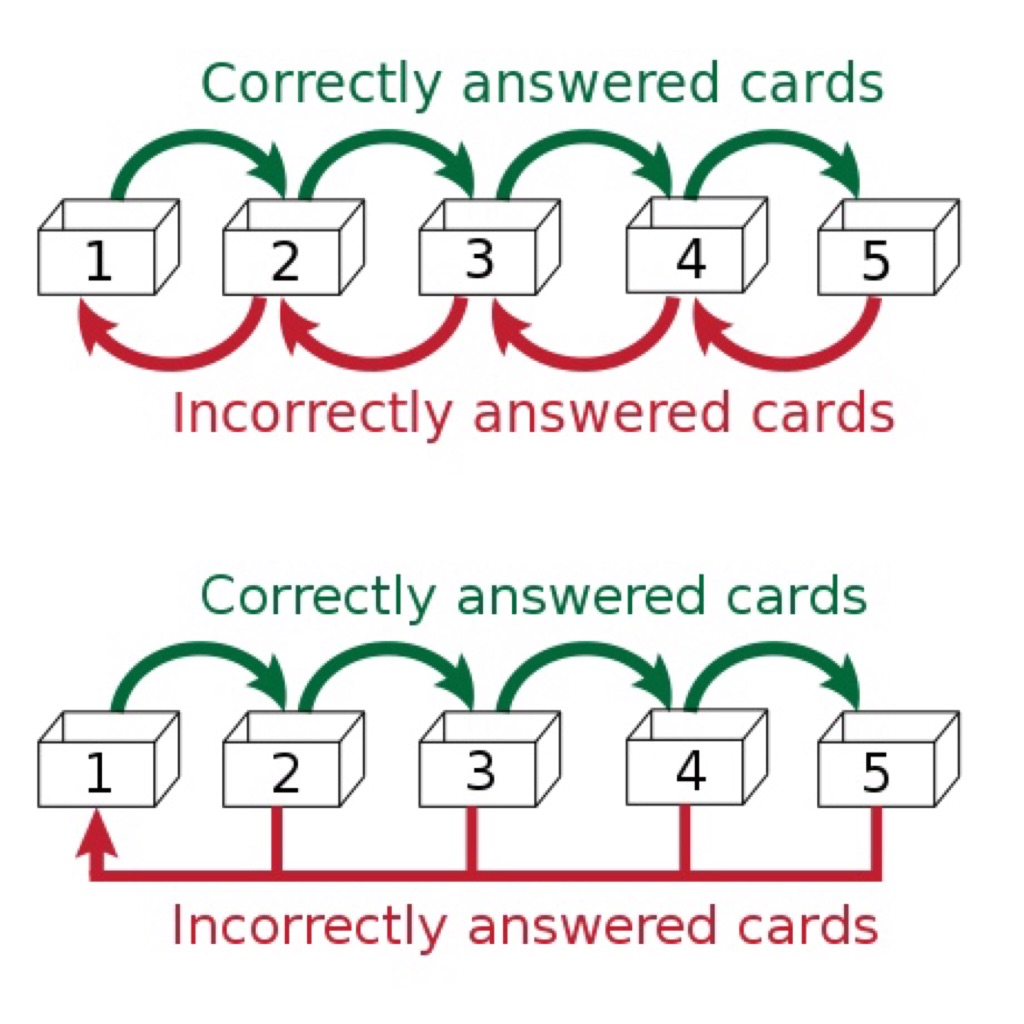
\includegraphics[width=0.50000\textwidth]{assets/leitner.jpg}
\caption{Two versions of the Leitner system for spaced repetition. Top:
The Leitner system where correctly answered flashcards are moved to the
next, less frequently practiced box, and incorrectly answered flashcards
are moved back one box. Bottom: Alternative Leitner system where
incorrect answers are moved all the way back to the first
box.}\label{fig:leitner}
\end{figure}

\subsubsection{Notable Spaced Repetition
Software}\label{notable-spaced-repetition-software}

Software that assist in doing spaced repetition is called \emph{spaced
repetition software} (SRS) and started to appear in the 1980s. The
benefit of having a digital system is that the tedious scheduling can be
done by an algorithms, whereas the physical system would be confined to
a small number of boxes using the Leitner system. Furthermore algorithms
can be adapted and improved. And most importantly digital systems
produces a lot of data that can be analyzed and studied for better
models of memory and scheduling.
\href{https://www.supermemo.com}{SuperMemo} developed by the Polish
researcher Piotr Wozniak was one of the first if its kind, and featured
an algorithm called SM2 (the latest version is SM-17). Wozniak was in
many ways a pioneer in the world of SRS\footnote{For the interested
  reader, I can highly recommend the piece from Wired back in 2012:
  https://www.wired.com/2012/01/everything-about-learning/}. SuperMemo
and it's generations of ``SM'' algorithms form the basis of the
algorithms of many other systems. This algorithm takes into account how
many times the flashcard has been seen, and the user input of how hard
it was to remember, and uses this to set an ideal review date for the
flashcard.

Notable examples are of SRS is
\href{https://www.duolingo.com}{Duolingo}\footnote{https://www.quora.com/Does-Luis-Von-Ahn-have-any-plans-for-optimizing-Duolingos-vocabulary-learning-using-spaced-repetition},
a popular app for learning languages, and
\href{https://www.memrise.com}{Memrise}, a similar app that in
additional to languages also have decks for more other topics.

Very popular choices for universal SRS applications are
\href{https://apps.ankiweb.net}{Anki} an
\href{https://mnemosyne-proj.org/}{Mnemosyne}, both popular because they
are free\footnote{Anki on iOS is the only application that costs money,
  to support the person behind Anki, but it's free on all other
  platforms.} and open source and available on all major platforms
(Windows, Mac, Linux, iOS\footnote{Mnemosyne doesn't have an iOS app.}
and Android). There are many more options for universal SRS
software.\footnote{For a table of flashcard software, see
  https://en.wikipedia.org/wiki/List\_of\_flashcard\_software} Mnemosyne
is especially interesting in that it's users can volunteer their data to
an open dataset that can then be studied for science. SuperMemo's second
iteration of its algorithm from 1987, SM2\footnote{https://www.supermemo.com/help/smalg.htm},
is notable because it's a very popular algorithm that is being used in
many other SRS, including Anki\footnote{Anki uses a slight modification
  of the SM2 algorithm: https://apps.ankiweb.net/docs/manual.html} and
Mnemosyne\footnote{https://mnemosyne-proj.org/principles.php}. But as we
shall see in a later section, more rigorous models than the heuristic SM
algorithms have been developed very recently, which no SRS that I'm
aware of have implemented yet\footnote{With the possible exception of
  \href{https://www.knewton.com}{Knewton} where the researcher was an
  intern as I understand it - but Knewton's product is not purely a SRS}.

\section{Spaced Repetition}\label{spaced-repetition}

Spaced repetition is a very well-documented phenomenon. A study in 2016
found that ``Hundreds of studies in cognitive and educational psychology
have demonstrated that spacing out repeated encounters with the material
over time produces superior long-term learning, compared with
repetitions that are massed together'', and also that ``spaced practice
is a feasible and cost-effective way to improve the effectiveness and
efficiency of learning, and has tremendous potential to improve
educational outcomes'' (Kang 2016).

The benefits, it turns out, goes beyond just memory. Spaced practice
enhances diverse forms of learning, including (Kang 2016):

\begin{itemize}
\tightlist
\item
  Memory
\item
  Problem solving
\item
  Generalization to new situations
\item
  Augmented learner metacognition
\end{itemize}

\subsection{Why Memorize at All?}\label{why-memorize-at-all}

(Kang 2016) writes:

\begin{quote}
Few would argue that memorizing instructional content, so as to be able
to reproduce the information verbatim from memory, is the ultimate goal
of education. Nonetheless, acquiring foundational knowledge and being
able to quickly access relevant information from memory are often
prerequisites for higher order learning and reasoning. For instance,
remembering arithmetic facts (e.g., times table) is a critical part of
mathematical skill learning, and a transition from calculation to direct
memory retrieval of the answer allows more efficient problem solving
(e.g., Siegler, 1988)

In short, spaced practice can improve students' memory for essential
facts and concepts, which in turn facilitates more complex learning and
problem solving.
\end{quote}

This fits well into the concepts that Dr.~Barbara Oakley and
Dr.~Terrence Sejnowski have popularized in the Coursera course
``Learning How To Learn''\footnote{https://www.coursera.org/learn/learning-how-to-learn},
and in Oakley's book ``A Mind for Numbers: How to Excel at Math and
Science'';\footnote{https://www.goodreads.com/book/show/18693655-a-mind-for-numbers}
namely:

\begin{enumerate}
\def\labelenumi{\arabic{enumi}.}
\tightlist
\item
  The limited capacity of working memory means that we can give
  attention to around 3--5 items at the same time.
\item
  The concept of ``chunking'' and ``chunks'' as units of informaton that
  is understood and stored in memory (short or long term).
\end{enumerate}

Studies have found that the capacity of the working memory naturally
differs to a small extend among people\footnote{https://www.coursera.org/learn/learning-how-to-learn},
and while it can be enhanced a little bit by training, there is a
fundamental limit: ``We found that by the end of day five\ldots{}their
working memory {[}capacity{]} had expanded from one to four items, but
not to five.''\footnote{http://www.apa.org/monitor/sep05/workout.aspx}.
Since working memory capacity is a fundamental limitation that we can't
do much about, we should try and make the best of the working memory
that we do have. Oakley describes how chunks of information can be
recombined and compounded into higher abstractions, corresponding to
higher levels of understanding. For example:

\begin{itemize}
\tightlist
\item
  We practice arithmetic until it becomes second nature, then offload
  the heavy calculations to a computer.
\item
  We practice matrix multiplication until it becomes second nature, and
  then use a computer.
\item
  We practice finding eigenvalues and eigenvectors of matrices until we
  become fluent in it. Afterwards we are comfortable talking about
  eigenvalues and eigenvectors when we encounter them in the myriad of
  applications in science and engineering.
\end{itemize}

Thus we would never get anywhere if we had to understand everything in
terms of the fundamentals everytime we needed to use a concept that is
composed of many simpler concepts; we simply wouldn't get anywhere.
Oakley herself places enormous weight on fluency\footnote{https://www.nytimes.com/2017/08/04/education/edlife/learning-how-to-learn-barbara-oakley.html}:

\begin{quote}
Chunks build on chunks, and, she says, the neural network built upon
that knowledge grows bigger. ``You remember longer bits of music, for
example, or more complex phrases in French.'' Mastering low-level math
concepts allows tackling more complex mental acrobatics. ``You can
easily bring them to mind even while your active focus is grappling with
newer, more difficult information.''
\end{quote}

In conclusion: fluency often comes before understanding. It is not our
objective to remember all the details of everything we learn, but to
achieve fluency in our craft, and remember the core of the teachings.

\subsection{How Effective Is Cramming?}\label{how-effective-is-cramming}

Since cramming is the most popular study technique by students (Kang
2016), it's worth to know just how effective is compared to spaced
practice, and how they differ.

And it turns out, cramming works! (Vacha and McBride 1993) That is why
students do it. But as (Branwen 2009) noted: ``Note that there is no
measure of long-term retention, suggesting that people who only care
about grades are rationally choosing to cram''.

The problem that massed practice leads to \emph{feelings} of fluency,
and since it \emph{can} work for increasing the task-performance in the
short term, which is all that matters at an exam, students frequently
rate massing as more effective than spacing (Branwen 2009):

\begin{quote}
Across experiments, \emph{spacing} was more effective than massing for
90\% of the participants, yet after the first study session, 72\% of the
participants believed that \emph{massing} had been more effective than
spacing\ldots{}.When they do consider spacing, they often exhibit the
illusion that massed study is more effective than spaced study, even
when the reverse is true.
\end{quote}

Ironically, it was repeatedly shown that low achievers in universities
cram the most (Branwen 2009):

\begin{quote}
We surveyed 324 undergraduates about their study habits as well as their
college grade point average (GPA). Importantly, the survey included
questions about self-testing, scheduling one's study, and a checklist of
strategies commonly used by students or recommended by cognitive
research. Use of self-testing and rereading were both positively
associated with GPA. Scheduling of study time was also an important
factor: Low performers were more likely to engage in late-night studying
than were high performers; massing (vs.~spacing) of study was associated
with the use of fewer study strategies overall; and all students-but
especially low performers-were driven by impending deadlines. Thus,
self-testing, rereading, and scheduling of study play important roles in
real-world student achievement.
\end{quote}

As Nate Kornell, a psychologist at Williams College, put it in an
interview with The New York Times, ``Forgetting is the friend of
learning'':

\begin{quote}
Cognitive scientists do not deny that honest-to-goodness cramming can
lead to a better grade on a given exam. But hurriedly jam-packing a
brain is akin to speed-packing a cheap suitcase, as most students
quickly learn - it holds its new load for a while, then most everything
falls out\ldots{}.When the neural suitcase is packed carefully and
gradually, it holds its contents for far, far longer. An hour of study
tonight, an hour on the weekend, another session a week from now: such
so-called spacing improves later recall, without requiring students to
put in more overall study effort or pay more attention, dozens of
studies have found.

``The idea is that forgetting is the friend of learning'', said
Dr.~Kornell. ``When you forget something, it allows you to relearn, and
do so effectively, the next time you see it.''

That's one reason cognitive scientists see testing itself - or practice
tests and quizzes - as a powerful tool of learning, rather than merely
assessment. The process of retrieving an idea is not like pulling a book
from a shelf; it seems to fundamentally alter the way the information is
subsequently stored, making it far more accessible in the future.
\end{quote}

With that out of the way, we will look at the two components of spaced
repetition.

\hypertarget{spaced-practice}{\subsection{Spaced
practice}\label{spaced-practice}}

\emph{Spaced practice} is studying the same material with some time in
between (at least 3--7 days) rather than immediately after (always same
or next day). The opposite is called massed practice.

The benefits of \emph{spaced practice} is better retention in the
longer-term. Thus the effect may not should up immediately as
illustrated in the following study:

\begin{quote}
One group of students heard the oath read 6 times in a row; another
group heard the oath 3 times on 1 day and 3 more times 3 days later. The
students recalled as much as they could immediately after hearing the
oath for the sixth time and again 4 weeks later. On the immediate test,
the group that received massed repetition recalled slightly more than
the group that received spaced repetition. But on the delayed test 4
weeks later, the spaced group clearly outperformed the massed group.
While massed practice might appear more effective than spaced practice
in the short term, spaced practice produces durable long-term learning
\end{quote}

Or as (Branwen 2009) puts it:

\begin{quote}
The spacing effect essentially says that if you have a question (``What
is the fifth letter in this random sequence you learned?''), and you can
only study it, say, 5 times, then your memory of the answer (``e'') will
be strongest if you spread your 5 tries out over a long period of time -
days, weeks, and months. One of the worst things you can do is blow your
5 tries within a day or two.
\end{quote}

The spacing effect appears to be so fundamental it can be found in:
extends to very different domains and even across species (Branwen
2009):

\begin{itemize}
\tightlist
\item
  Various domains, such as learning perceptual motor skills, learning
  lists of words etc.
\item
  Across species: Humans, rats, pigeons, flies, bumblebees, seaslugs.
\item
  Across age groups: infancy, childhood, adulthood, the elderly and
  individuals with various memory impairments.
\item
  Across retention intervals of seconds, days, months, even years.
\end{itemize}

Read (Branwen 2009) for more details and how spaced practice compares in
different domains, in particular how increased lags between practices
affects performance.

\begin{quote}
Overall, Donovan and Radosevich found that increasingly distributed
practice resulted in larger effect sizes for verbal tasks like free
recall, foreign language, and verbal discrimination, but these tasks
also showed an inverse-U function, such that very long lags produced
smaller effect sizes.

In contrast, increased lags produced smaller effect sizes for skill
tasks like typing, gymnastics, and music performance.
\end{quote}

Concluding (emphasis added by me):

\begin{quote}
Skills like gymnastics and music performance raise an important point
about the testing effect and spaced repetition: \textbf{they are for the
maintenance of memories or skills, they do not increase it beyond what
was already learned. If one is a gifted amateur when one starts
reviewing, one remains a gifted amateur.}
\end{quote}

We are here again reminded of the important distinction between
learning/understanding and memorizing/practicing.

\subsubsection{Why Does Spaced Practice
Work?}\label{why-does-spaced-practice-work}

There are a number of theories:

\begin{enumerate}
\def\labelenumi{\arabic{enumi}.}
\tightlist
\item
  One of the most prominant ones is that repeating an item reminds the
  learner of it's prior occurance, which triggers retrieval of the past
  internal representation of the item and it's context. This retrieval
  process enhances and reinforces the memory by strengthening the old
  neural pathsways of that memory. Massed repetition eliminates the
  retrieval process---there is no need to retrieve from memory because
  the same item was just presented (Kang 2016). This is closely related
  to the \emph{testing effect}:
\end{enumerate}

\begin{quote}
\textbf{The
\href{https://en.wikipedia.org/wiki/testing\%20effect}{testing effect}}
is the established psychological observation that the mere act of
testing someone's memory will strengthen the memory (regardless of
whether there is feedback). Since
\href{https://en.wikipedia.org/wiki/spaced\%20repetition}{\textbf{spaced
repetition}} is just testing on particular days, we ought to establish
that testing works better than regular review or study, and that it
works outside of memorizing random dates in history.
\end{quote}

\begin{enumerate}
\def\labelenumi{\arabic{enumi}.}
\setcounter{enumi}{1}
\tightlist
\item
  Another theory emphasizes the learning context (what surrounds an
  event, from the external environment to an individual's mental state).
  With spaced repetitions, the creations of new associations and
  contexts to the same item may take place, giving multiple ``paths''
  the retrieve the same memory (Kang 2016) and (Branwen 2009).
\item
  And finally, another theory points to the fact that the attention of a
  student decrease when it is perceived that the presented information
  is already known.
\end{enumerate}

The different theories (retrieval of memory enhancing it, new contexts
being made with a memory and redudancy reducing attention), are not
mutually exclusive, and multiple mechanisms may act in concert to yield
the memory advantage produced by spaced practice (Kang 2016).

\hypertarget{self-testing}{\subsection{Self-testing}\label{self-testing}}

\emph{Self-testing} or \emph{retrieval} is trying to recall information
from memory instead of passively re-studying it. The benefits of
retrieval was found to boost learning in various ways (Kang 2016):

\begin{itemize}
\tightlist
\item
  Improved memory for the tested information
\item
  Slowed forgetting
\item
  Transfer of learning to new situations
\item
  Generalization to new examples
\item
  Potentiated subsequent learning
\item
  Augmented learner metacognition
\end{itemize}

A particularly interesting finding is that self-testing does not only
improve \emph{memory} but also \emph{generalization}, i.e.~the student's
ability to apply the knowledge in new situations.

\begin{quote}
This review has so far focused on how spaced practice improves memory,
in part because memory researchers first observed the spacing effect and
also because the majority of prior studies examined memory.
\textbf{Although acquiring and retaining knowledge matters in education,
a more crucial objective is transfer, the ability to utilize what was
learned to answer new questions or solve new problems (after all, in
real life the likelihood of encountering material in exactly the same
way as presented during instruction is exceedingly low)}. Mere
remembering of content is rote learning, focused on the past; on the
contrary, meaningful learning involves transfer and orients toward the
future (Mayer, 2002).

Although the research surrounding the benefits of spaced practice for
more complex kinds of learning is not as extensive as that for memory,
some evidence indicates that spacing can enhance meaningful learning
that generalizes to new situations (see Carpenter, Cepeda, Rohrer, Kang,
\& Pashler, 2012, for a review). In one study, college students attended
a 45-min lecture on meteorology and then reviewed the information (in a
quiz with corrective feedback) either 1 or 8 days later (Kapler, Weston,
\& Wiseheart, 2015). On a final test 35 days after the review session,
students in the 8-day condition performed better than those in the 1-day
condition not just on the factual recall questions but also on the
questions that required application of knowledge. Other studies support
spaced practice of mathematics problems (Rohrer \& Taylor, 2006) and
ecology lessons (Gluckman, Vlach, \& Sandhofer, 2014; see also Vlach \&
Sandhofer, 2012). In addition to improving mathematics problem solving
and science concept learning, spaced practice benefits the long-term
learning of English grammar in adult English-language learners (Bird,
2010). \textbf{In all cases, the students were not just memorizing
solutions but were instead applying their learning to solve new
problems.}
\end{quote}

Regarding the type of self-testing that works best, (Branwen 2009) found
by literature review:

\begin{quote}
The research favors questions which force the user to use their memory
as much as possible; in descending order of preference:

\begin{enumerate}
\def\labelenumi{\arabic{enumi}.}
\tightlist
\item
  free recall
\item
  short answers
\item
  multiple-choice
\item
  Cloze deletion
\item
  recognition
\end{enumerate}
\end{quote}

\subsubsection{Downsides to
Self-testing}\label{downsides-to-self-testing}

The downsides to self-testing are minor, but worth mentioning (Branwen
2009):

\begin{enumerate}
\def\labelenumi{\arabic{enumi}.}
\tightlist
\item
  \textbf{Interference in recall}, where ability to remember tested
  items drives out ability to remember similar untested items. But
  ``\emph{At worst, interference of this sort might dampen positive
  testing effects somewhat. However, the positive effects of testing are
  often so large that in most circumstances they will overwhelm the
  relatively modest interference effects.}''
\item
  \textbf{Multiple choice tests can accidentally lead to ``negative
  suggestion effects''}, where a previously seen falsehood makes one
  more likely to believe it. But ``This is mitigated or eliminated when
  there's quick feedback about the right answer''.
\end{enumerate}

So we won't worry much about either; the first we won't worry about
there is nothing to do about it and reportedly the benefits outweigh the
downside, and the second we can make sure to counter by ensuring
immediate feedback.

\subsection{Spaced Repetition = Testing +
Spacing}\label{spaced-repetition-testing-spacing}

It was found that the two strategies of retrieval and spacing combined
to amplify the benefits of each (Kang 2016). Thus we can say:

\textbf{Testing + Spacing = Spaced repetition}

\subsection{Dynamics of Reviewing Similar
Memories}\label{dynamics-of-reviewing-similar-memories}

(Subirana, Bagiati, and Sarma 2017) brought up a question that is still
partially unaddressed in the literature: when is a memory ``refreshed''
or ``practiced'', that is, when should we reset the clock to zero?:

\begin{quote}
If we review derivatives, are we also implicitly reviewing integrals? If
we review how the Pythagoras theorem can be derived, are we also
reviewing how it can be applied?
\end{quote}

This question I do think we should be able to answer through data
analysis of a suitably designed SRS such as the one proposed in this
report. The little evidence there is seem to suggest both that reviewing
concept do \emph{somewhat} transfer to related concepts, and also that
other factors such as practical application of knowledge and emotional
impact may be important (Subirana, Bagiati, and Sarma 2017):

\begin{quote}
Direnga et al {[}42{]} showed that members active in the subject show
improvements which may mean that Ebbinghaus speed does not applied if
``similar'' concepts are reviewed. Fritz et al {[}43{]} tested retention
over a 6-month period and found using a simple model to explain a
concept is equal to a sophisticated model in terms of retention of
medical instruction suggesting other factors, such as emotional impact,
are essential to retention.
\end{quote}

\subsection{When to Use Spaced
Repetition}\label{when-to-use-spaced-repetition}

Based on empirical findings by Piotr Wozniak\footnote{https://www.supermemo.com/articles/programming.htm}
and some back of the envelope calculations, Gwern arrived at
rule-of-thumb (Branwen 2009):

\begin{quote}
5 minutes is the line that divides trivia from useful data. (There might
seem to be thousands of flashcards that meet the 5 minute rule. That's
fine. Spaced repetition can accommodate dozens of thousands of cards).
\end{quote}

What if one is in a hurry for an exam? (Branwen 2009) estimates:

\begin{quote}
To a lesser extent, one might wonder when one is in a hurry, should one
learn something with spaced repetition and with massed? How far away
should the tests or deadlines be before abandoning spaced repetition?
It's hard to compare since one would need a specific regimens to compare
for the crossover point, but for massed repetition, the average time
after memorization at which one has a 50\% chance of remembering the
memorized item seems to be 3-5 days. Since there would be 2 or 3
repetitions in that period, presumably one would do better than 50\% in
recalling an item. 5 minutes and 5 days seems like a memorable enough
rule of thumb:

\textbf{``Don't use spaced repetition if you need it sooner than 5 days
\emph{or} it's worth less than 5 minutes''.}
\end{quote}

I will note that these results are only strictly applicable to
standalone-facts, where it's all about the space-time tradeoff\footnote{https://en.wikipedia.org/wiki/Space--time\_tradeoff},
but does not necessarily apply to highly interrelated information that
is ``chunked'' to achieve higher abstraction levels.

\pagebreak

\section{Challenges and Tips for Spaced
Repetition}\label{challenges-and-tips-for-spaced-repetition}

By broad survey I have found the most common complaints and mistakes
with spaced repetition to be:

\begin{itemize}
\item
  \textbf{Formulating poor questions and answers} (Branwen 2009)
\item
  \textbf{Memorizing before learning:} Assuming it will help you learn,
  as opposed to maintain and preserve what one already learned. It's
  hard to learn \emph{from} cards, but if you have learned something,
  it's much easier to then devise a set of flashcards that will test
  your weak points. (Branwen 2009)
\item
  \textbf{Loss of context:} Flashcards are less useful to learning the
  ``big picture''. If you are memorizing a large amount of information,
  there is often a hierarchy, organization, etc that can make leaning
  the whole thing easier, and you loose the constant visual reminder of
  the larger context when using flashcards.\footnote{A user on
    LessWrong.com used Flashcards extensively for 3 years in medical
    school, and after failing to receive any substantial benefits and
    meeting with a learning-skills specialist, wrote an article about
    it:
    http://lesswrong.com/lw/juq/a\_vote\_against\_spaced\_repetition/}
\item
  \textbf{Flashcards not taking advantage of spatial, mapping, or visual
  memory}, all of which the human mind is much better optimized for. It
  is not so well built to memorize pairs between seemingly arbitrary
  concepts with few to no intuitive links. My preferred methods are, in
  essence, hacks that use your visual and spatial memory rather than
  rote.\footnote{A user on LessWrong.com used Flashcards extensively for
    3 years in medical school, and after failing to receive any
    substantial benefits and meeting with a learning-skills specialist,
    wrote an article about it:
    http://lesswrong.com/lw/juq/a\_vote\_against\_spaced\_repetition/}
\item
  \textbf{Overload:} Feelings of overwhelm as the daily flashcard review
  number becomes too big.
\end{itemize}

Some of the problems there are definite remedies against, and some there
is still somewhat lack of in-depth studies. We will now address the
problems listed above.

\subsection{General Tips for Flashcard
Creation}\label{general-tips-for-flashcard-creation}

Piotr Wozniak, the Polish scientist behind SuperMemo, is the author is a
webpage ``Effective learning: Twenty rules of formulating
knowledge''\footnote{https://www.supermemo.com/en/articles/20rules} that
in my experience is one of the most cited lists of good flashcard
creation practices.

Here is my interpretation of the most important ones:

\begin{itemize}
\tightlist
\item
  \textbf{Learn before you memorize} - you need to build an overall
  picture of the learned knowledge. \emph{Remember: it's spaced
  repetition, not spaced learning}.
\item
  \textbf{Make cards minimal} - break down the information to the
  simplest chunks that still makes sense, instead of filling the card
  with multiple facts.
\item
  \textbf{Use imagery} - to involve our visual cortex, which is strongly
  associated with memory.
\item
  \textbf{Use mnemonic techniques} - take advantage of the brain's
  natural power to remember quirky things and stories - the more crazy
  and memorable the better.
\item
  \textbf{Rely on emotional states} - Use objects that evoke very
  specific and strong emotions: love, sex, war, your late relative,
  object of your infatuation - it is well known that emotional states
  can facilitate recall.
\item
  \textbf{Refer to other memories} - Can place your item in a better
  context, simplify wording, and reduce interference.
\end{itemize}

This list can be extended with what I believe are good heuristics around
making flashcard, form own experience and reading other people's
experience:

\begin{itemize}
\tightlist
\item
  \textbf{Make your own flashcards}
\item
  \textbf{Only include the most important} - Use 80/20 rule to narrow
  down the best stuff.
\item
  \textbf{Don't make flashcards immediately} - Be careful to make
  flashcards on the run, while learning the material. It is often more
  effective first apply the concept a few times first, rather than
  having to rewrite almost every flashcard.
\item
  \textbf{Why questions} - Cards that answer the question ``Why?'' are
  more valuable than factual cards.
\item
  \textbf{Say your answers loud when studying} - has been confirmed by
  recent study to work (Forrin and MacLeod 2017)
\item
  \textbf{Study your flashcards in both directions} - meaning that both
  sides of the card can act like question and answer.
\item
  \textbf{Don't treat flashcard like a silver bullet} - Write an
  explanation in your own words, create a quiz, take a practice test
  written by someone else, work lots of practice problems (your go-to
  strategy for math), make mind maps or Venn diagrams etc.\footnote{https://collegeinfogeek.com/flash-card-study-tips/}
\item
  \textbf{Don't practice mindlessly} - Actively trying to retrieve
  memories is more important than finishing quickly.
\item
  \textbf{Don't study in one big session} - Use you small windows of
  time, e.g.~the bus stop, time between classes etc.
\end{itemize}

For good lists of tips see.\footnote{http://rs.io/anki-tips/}\footnote{https://collegeinfogeek.com/flash-card-study-tips/}\footnote{http://skillcookbook.com/flashcards/}

\hypertarget{the-question-of-context}{\subsection{The Question of
Context}\label{the-question-of-context}}

Is there a loss of context, or \emph{hindering of abstraction} with the
use of flashcard? This is one of the most important and legitimate
questions about flashcards in my opinion. The usage of spaced repetition
is straight forward when it comes to simple facts. In fact,
``\href{https://en.wikipedia.org/wiki/Roger\%20Craig\%20\%28Jeopardy\%21\%20contestant\%29}{Robert
Craig} set multiple records on the quiz show
\href{https://en.wikipedia.org/wiki/Jeopardy\%21}{\emph{Jeopardy!}}
2010-2011 in part thanks to
\href{http://quantifiedself.com/2011/09/roger-craig-on-knowledge-tracking/\#comment-3004}{using
Anki} to memorize chunks of a collection of
\href{http://www.j-archive.com/}{\textgreater{}200,000} past questions;
a later Jeopardy winner, Arthur Chu, also used spaced repetition''
(Branwen 2009).

However things are not so simple with concept on a higher level than
simple facts (Branwen 2009):

\begin{quote}
{[}A{]} potential objection is to argue that spaced repetition
inherently hinders any kind of abstract learning and thought because
related materials are not being shown together - allowing for comparison
and inference - but days or months apart. Ernst A. Rothkopf: ``Spacing
is the friend of recall, but the enemy of induction'' (Kornell \& Bjork
2008, p.~585). This is plausible based on some of the early studies but
the 4 recent studies I know directly examining the issue both found
spaced repetition helped abstraction as well as general recall:
\end{quote}

Like Gwern, I also found most newer papers optimistic, such as
(Subirana, Bagiati, and Sarma 2017), but I also have my own take on
this.

I think this is a really important subject, if one wish to apply spaced
repetition to fields such as science and engineering. I have personally
experienced limits to the effectiveness of the SRS system Anki during my
own experiements with it, and it needs to be addressed.

My answers is that here needs to be:

\begin{enumerate}
\def\labelenumi{\arabic{enumi}.}
\tightlist
\item
  \textbf{A concept of closely related flashcards that logically makes
  sense to group together when reviewing flashcards on that particular
  subject.} The user should have granular control over the size of these
  clusters. Logically there should be an optimum; too small clusters
  (down to single cards), and the flashcard review can feel too
  unfocused and not enough emphasis is put on the links between
  flashcards. Too big clusters, and the benefits of interleaving is
  likely to be lost, and there is a risk of the student receiving too
  many hints to various flashcards instead of retrieving from memory. I
  have not been able to find any rigorous studies on the effectiveness
  on various sizes of these relatedness-clusters, and it's clear that
  more studies are needed. Such as study would be helped immensely by
  the data that would be generated from the proposed learning platform
  that is the subject of this report.
\item
  \textbf{A concept of dependency, i.e.~a mechanism to present certain
  cards before others could be tested}. It's not a given that a
  particular order / dependency is needed of there is a concept of a
  related set of cards, but it's an option that should be studied.
\end{enumerate}

As reviewed earlier, our minds use chunks and clusters. You want as many
connections to each fact.

One thing must be noted in about tip on making cards minimal; not all
subjects are ``coercive to flashcards'' or some would say
``flashcard-eligible''. As user noted\footnote{reviewing-thinking}:

\begin{quote}
\textbf{Not all subjects are flashcard-eligible}. You need to be aware
of that. Memorizing chapters of a book by making flashcards is one of
the least effective ways of remembering the content of those chapters as
a whole. Trying to recall the content while giving little explanations
as if you're giving a lecture is a far more effective way to do it. And
I always get something different every time I read the same book. Anki
only tells me when I'm about to forget that, and if I wanted to retain
that knowledge, I'd better review it decently.

\textbf{Your cards must act as indexes.} Your brain should be an index.
Every time that I begin to make too much mistakes on certain flashcards,
it's CLEAR that you're not remembering because you DIDN'T learn it
correctly in the first place, not because anything else. So you mark
that card, go back and review your book, lecture, notes, resource and
make a couple more flashcards of that tiny bit that you're getting wrong
every time.
\end{quote}

Another user also resisted the idea of flashcard necessarily being
completely broken down, atomized pieces of information\footnote{https://yourawesomememory.com/content/reviewing-thinking}:

\begin{quote}
\textbf{Use a card to remind you to think}

For decks with higher level concepts like Algorithms or Game theory
every time I review a card I explain it and I let me my mind linger and
come up with associations. It's rare the card where at least 1 or 2
associations new associations don't pop in my mind including questions.
Besides that it's also usually the case that when I try to explain a
concept I find little nuances or questions that I then research. And
that builds new associations too.

This requires time, of course, that's why I find it important to prune
knowledge aggressively. I am generally eager to add new knowledge and
overestimate its value.
\end{quote}

So instead of treating flashcards merely as a ``game'' of getting a high
retrieval score. ``Instead, whether I happen to have perfect recall or
not, I should focus on: `This is my time to \emph{think about this
again}.'\footnote{https://yourawesomememory.com/content/reviewing-thinking}Many
users in STEM fields, have found flashcards to be useful simply for
triggering a whole network of association around a concept, due to the
nature of the highly interconnected concepts in STEM:

\begin{quote}
\textbf{I'm a Human, Not a~Computer} Computers can't think. But they can
copy terabytes of data in a few~minutes. If I view Anki as copying data
into my brain, it will drive me nuts that it takes so many hours to copy
so few bits of data. It makes me feel like a shoddy, vacuum-tube
prototype mainframe that keeps chewing up its~punchcards. But if I view
Anki as triggering thoughts, awakening whole networks of experiences and
associations, then remembering will make me more human. I won't review
for the sake of awesome, high-quality thinking later. My reviews will be
that high-quality thinking. Right~now.
\end{quote}

The people behind SuperMemo regularly responds to critique in
\href{http://supermemopedia.com}{their wiki}. In response to the
particular critique about not being able to maintain ``the big picture''
in an SRS system, they responded\footnote{http://supermemopedia.com/wiki/A\_vote\_against\_spaced\_repetition}:

\begin{quote}
The argument that SuperMemo does not hold the ``big picture'' is as old
as SuperMemo. The answer is always the same: you do not need the big
picture in SuperMemo as long as you keep it in your head. Many students
fail this principles and their effectiveness in using spaced repetition
is also undermined.

Students may give up spaced repetition at their own peril. Without
review, memories disappear. Spaced repetition helps minimize the review.
However, the entire process relies heavily on smart learning, right
choices, material selection, item formulation, and other learning
strategies.

Smart learning is difficult because it requires that you be \ldots{}
well \ldots{} smart.
\end{quote}

\subsection{Overload}\label{overload}

Many users of SRS report being overwhelmed by the system. It could be
that they add a lot of trivial things they don't care about, or that
they add relevant stuff but too fast.

This point will be addressed in the section
``\protect\hyperlink{paper-summary-on-optimizing-spacing-schedule}{Paper
Summary on Optimizing Spacing Schedule}'' where model for optimal inflow
rate of new cards is developed.

\pagebreak

\hypertarget{interleaved-practice}{\section{Interleaved
Practice}\label{interleaved-practice}}

We briefly touched upon \emph{interleaved practice} in section
``\protect\hyperlink{what-works}{What Works}'' i.e.~learning
\texttt{AAABBBCCC\ vs\ ABCABCABC}.

Studies of interleaved practice shows most improvement of learning in
mathematical knowledge (Kang 2016). It makes sense that subjects in
science and engineering is where interleaved practice really shines
because forces the student into thinking about a broader range of
learned concepts and which one to apply (and why), instead of knowing
that this problem must belong to a certain chapter. Therefore
interleaved practice makes the learning situation more similar to an
actual exam or even real-life application.

Interleaving has also shown to benefit in fields of category
discrimination such as recognition and classification of art (Kang
2016). ``Students after blocked practice had difficulty discriminating
among the problem types and knowing when to use which formula.
Therefore, similar to category learning, interleaved practice seems to
help learners differentiate among the types of problems they are
learning to solve'' (Kang 2016).

It has also been suggested that attentional lapses can play a role. A
study found that mind wandering is more likely during blocked than
interleaved training (Kang 2016). When presented with material that is
completely different, the mind is less likely to wonder.

\begin{center}\rule{0.5\linewidth}{\linethickness}\end{center}

In conclusion, ``\textbf{multiple mechanisms may underlie the
interleaving advantage: Attention, temporal spacing, and juxtaposing
different categories could jointly contribute to learning}.'' (Kang
2016)

Where does interleaved practice fit into a SRS flashcard system? Quite
simply, reviewing flashcards is inherently interleaved, to the degree
one chooses not to group related cards together for review (see
discussion in section \protect\hyperlink{the-question-of-context}{The
Question of Context}).

Finally I will briefly mention that some very promising studies have
been done on using interleaved in the classroom simply by reorganizing
the homework assignments, which could be sufficient to produce sizable
gains! This is research I wish DTU would recognize and start to
implement on an experimental basis. I quote and emphasize the relevant
section in Appendix \ref{sec:classroom}.

\pagebreak

\hypertarget{optimal-spacing-schedule-for-spaced-repetition}{\section{Optimal
Spacing Schedule for Spaced
Repetition}\label{optimal-spacing-schedule-for-spaced-repetition}}

Robert Bjork\footnote{https://www.psych.ucla.edu/faculty/page/bjork} in
his 2012 Wired interview (``Everything You Thought You Knew About
Learning Is Wrong'' 2012):

\begin{quote}
The spacing effect was one of the proudest lab-derived discoveries, and
it was interesting precisely because it was not obvious, even to
professional teachers. The same year that Neisser revolted, Robert
Bjork, working with Thomas Landauer of Bell Labs, published the results
of two experiments involving nearly 700 undergraduate students. Landauer
and Bjork were looking for the optimal moment to rehearse something so
that it would later be remembered. Their results were impressive: The
best time to study something is at the moment you are about to forget
it. And yet --- as Neisser might have predicted --- that insight was
useless in the real world. Determining the precise moment of forgetting
is essentially impossible in day-to-day life.
\end{quote}

While it is an impossible task to determine this moment precisely for
everything we wish to remember, some progress has been made recently.

\subsection{Single Review Opportunity}\label{single-review-opportunity}

Let's start with the simplest situation: Given that you know the test
date, and you have a single review opportunity, when should you use it?
Of course, reviewing the test the same day, or day before the final test
would probably always give the best results on the test. But given what
we have established about the benefits of spaced practice, it is more
interesting to look at this question while subject the constraint that
there is always being a gap between review session and test session of
at least 7 days, which is what the following study did.

A large experiment examined 10 different lags (the spacing between
initial learning and retrieval practice review, that ranged from 0 to
105 days) and four different retention intervals. The final test was
administered either 7, 35, 70, or 350 days \emph{after} the review
session. **They found that retention was highest ``when the lag was
about 10\% to 20\% of the tested retention interval.** In other words,
there is no fixed optimal lag---It depends on the targeted retention
interval. If you want to maximize performance on a test about 1 week
away, then a lag of about 1 day would be optimal; but if you want to
retain information for 1 year, then a lag of about 2 months would be
ideal.''(Kang 2016). This comes with the ceveat that this was study
material was trivia facts, but it gives a sense of a ballpark figure.

\subsection{Multiple Review
Opportunity}\label{multiple-review-opportunity}

When you have multiple review opportunities, the natural question
becomes: what if you want to optimize a review schedule for
\emph{mastering} the maximum amount of information for the long term,
given some time constraints, rather than just optimize for a test on a
specific date?

As we have established, spacing out the multiple review opportunities
produces better learning than massing them together. There has been some
debate as to whether the multiple reviews should be spaced out
uniformly, or in an expanding schedule (meaning the lag progressively
increasing between each review). Most of the sources I have found
suggest an expanding schedule to be most effective, including (Kang
2016) and (Branwen 2009).

We shall look at a recent paper where an effort was made to put multiple
review spacing schedule in a more rigorous mathematical framework, use
data analysis as a means of memory model selection, and Amazon
Mechanical Turk to verify the findings.

\hypertarget{paper-summary-on-optimizing-spacing-schedule}{\subsection{Paper
Summary on Optimizing Spacing
Schedule}\label{paper-summary-on-optimizing-spacing-schedule}}

This section will go summarize the findings in the paper ``Unbounded
Human Learning: Optimal Scheduling for Spaced Repetition'' (Reddy et al.
2016) due to it's importance, and for including some of the latest
technical work in this area. It is the most technical section in this
report and the best attempt at a rigorous mathematical model I have seen
so far, with the ultimate goal of deciding the optimal frequency with
which new cards should be introduced into a flashcard deck to order to
optimize the ``throughput'' of flashcards, i.e.~number of mastered
flashcards per unit time, within some constraints of study time. I
recommend reading the full paper for anyone interested in the
mathematical modeling of memory and spaced repetition.

They make three contributions:

\begin{enumerate}
\def\labelenumi{\arabic{enumi}.}
\tightlist
\item
  \textbf{Mining large-scale log data to validate human memory models:}
  They perform observational studies on a user data from the Mnemosyne
  SRS application, with a dataset containing 859,591 interactions, 2,742
  users, and 88,892 items.
\item
  \textbf{Mathematical modeling of optimal spacing schedule}, by
  embedding above memory model into a stochastic model using \emph{queue
  theory}, and verifying by running simulations. As an aside, the main
  author have also modeled this using a neural network to do
  \emph{reinforcement learning} in another more recent paper (Reddy,
  Levine, and Dragan, n.d.). I will not to into detail with the
  reinforcement learning approach here since I have not had time to
  study it in-depth yet.
\item
  \textbf{Verification of the mathematical model in controlled
  experiments}, by hiring people on Amazon's
  \href{https://www.mturk.com/mturk/welcome}{Mechanical Turk}.
\end{enumerate}

\subsubsection{Paper Introduction}\label{paper-introduction}

\begin{quote}
Existing schemes for assigning review frequencies to different decks are
based on heuristics that are not founded on any formal reasoning, and
hence, have no optimality guarantees. One of our main contributions is a
principled method for determining appropriate deck review frequencies.

The problem of deciding how frequently to review different decks in the
Leitner system is a specific instance of the more general problem of
review scheduling for spaced repetition software. The main challenge in
all settings is that schedules must balance competing priorities of
introducing new items and reviewing old items in order to maximize the
rate of learning. While most existing systems use heuristics to make
this trade-off, our work presents a principled understanding of the
tension between novelty and reinforcement.
\end{quote}

\subsubsection{1: Testing Human Memory
Models}\label{testing-human-memory-models}

This section seeks to fit variations of a standard exponential
forgetting curve model, where recall is binary (user is assumed to
either completely recall or forget an item), and the probability of
recalling an item has the following function form: \[
P(\text{recall}) = \exp{(-\theta \cdot d/s)}.
\] They use a 0-Parameter and 1-Parameter Logistic Item Response Theory
models (0PL-IRT, 1PL-IRT) + a logistic regression model as benchmark
models, and compare 10 different exponential decay models containing
various combinations of the variables:

\begin{itemize}
\tightlist
\item
  \(d_{ij}\) as the time elapsed since previous review of item \(i\) by
  user \(j\).
\item
  \(q_{ij}\) for position (i.e.~deck number) of item \(i\) in Leitner
  system for user \(j\).
\item
  \(n_{ij}\) as the number of past reviews of item \(i\) by user \(j\).
\item
  \(\theta\) as a global item difficulty, i.e.~assuming that all items
  are equally difficult to memorize.
\item
  \(\theta\) as a item-specific difficulty, i.e.~we assume that some
  items may be easier to forget than others.
\end{itemize}

All other models are trained using maximum-likelihood estimation, and
they follow all the usual practice of cross validation.

Observations:

\begin{enumerate}
\def\labelenumi{\arabic{enumi}.}
\tightlist
\item
  \textbf{Positive impact of delay terms: }Models with delay term
  \(d_{ij}\) (time elapsed since last review) perform better than models
  without it.
\item
  \textbf{Use of item-specific difficulties:} Item-specific difficulties
  \(\theta_i\) outperforms global difficulty \(\theta\). However, they
  end up using global difficulty ``due to considerations of practicality
  (\(\theta_i\) may be unknown and/or difficult to estimate) and
  mathematical tractability''
\item
  \textbf{Leitner position \textgreater{}\textgreater{} number of
  reviews \textgreater{}\textgreater{} constant memory strength:
  }Setting memory strength \(s\) equal to Leitner deck position
  \(q_{ij}\) performs better than it proportional to the number of past
  reviews \(n_{ij}\), which in turn is better than using a constant
  \(s\).
\item
  \textbf{Performance comparable to best logistic regression model
  }Setting memory strength s equal to Leitner deck position \(q_{ij}\)
  performs better than it proportional to the number of past reviews
  \(n{_ij}\), which in turn is better than using a constant s.
\end{enumerate}

\subsubsection{2: A Stochastic Model for Spaced Repetition
Scheduling}\label{a-stochastic-model-for-spaced-repetition-scheduling}

Where the second section of the paper sought to find a suitable model of
human memory, the third section seeks to find an optimal scheduling
strategy for flashcards in the Leitner system, based on the memory model
from the previous section. A Leitner system was modelled using queuing
theory, see Fig.~\ref{fig:leitner-paper}. \textbf{In this model, a card
is considered to be mastered when it is successfully recalled at the
last card deck \(n\)} (in Fig.~\ref{fig:leitner-paper} that is deck 5).

And most crucially, it's assumed that the learner has a review frequency
budget (e.g., the maximum rate at which the user can review items) of
\(U\), which is to be divided between reviewing the decks as well as
viewing new items.

\begin{figure}
\centering
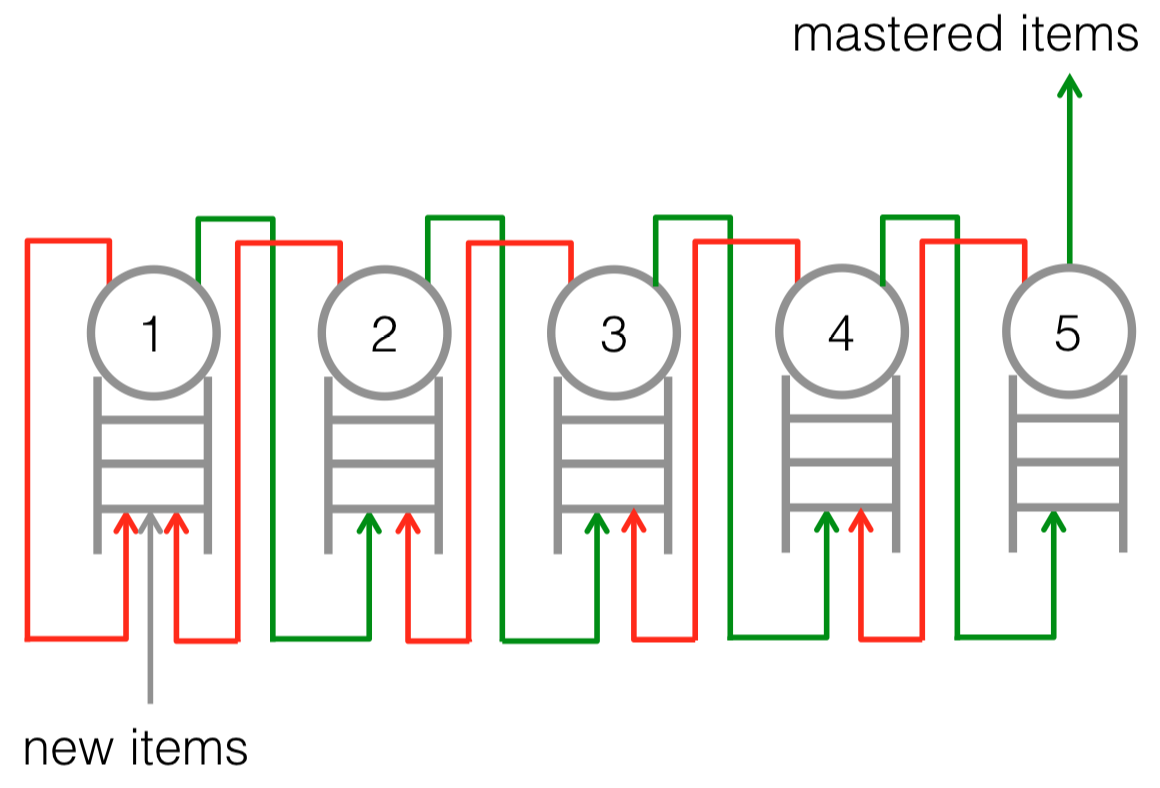
\includegraphics[width=0.65000\textwidth]{assets/leitner-paper.png}
\caption[The Leitner Queue Network: Each queue represents a deck in the
Leitner system. New items enter the network at deck 1. Green arrows
indicate transitions that occur when an item is correctly recalled
during review, and red arrows indicate transitions for incorrectly
recalled items. Queue k is served (i.e.~chosen for review) at a rate
\(\mu_k\), and selects items for review in a FIFO manner.]{The Leitner
Queue Network: Each queue represents a deck in the Leitner system. New
items enter the network at deck 1. Green arrows indicate transitions
that occur when an item is correctly recalled during review, and red
arrows indicate transitions for incorrectly recalled items. Queue k is
served (i.e.~chosen for review) at a rate \(\mu_k\), and selects items
for review in a FIFO manner.\footnotemark{}}\label{fig:leitner-paper}
\end{figure}
\footnotetext{Figure text taken from paper (Reddy et al. 2016)}

The learning rate \(\lambda_{out}\) is defined to be the long-term rate
of mastered items exiting from deck \(n\), i.e.: \[
\lambda_{out} = \lim_{T \rightarrow \infty} \frac{1}{T} \cdot \left|\{\text{Items mastered in interval } [0, T ]\}\right| 
\] The aim of a scheduling policy is to maximize \(\lambda_{out}\).

It is assumed that new items are injected into deck 1 following a
Poisson process with a chosen rate \(\lambda_{ext}\) (``arrival rate''),
and for each deck \(k\), we choose a ``service rate'' \(\mu_k\), which
represents the rate at which items from that deck come up for review. We
need to enforce that the arrival rate \(\lambda_{ext}\) and deck service
rates together satisfy the user's review frequency budget constraint,
i.e., \(\lambda_{ext} + \sum\limits_{k} \mu_k \leq U\). The problem is
then to choose the decision variables, arriaval rate \(\lambda_{ext}\)
and service rates \(\mu_k\), such that the learning rate
\(\lambda_{out}\) is maximized.

I won't go into details here, but in summary the strategy was the
following: a vector state was defined for each deck, forming a Markov
chain and finally using a so-called ``mean-recall approximation'' to
reduce the problem to a low-dimensional deterministic optimization
problem.

The primary qualitative finding to come out of this paper is a partiular
property of the optimal review schedule of a Leitner Queue Network
(LQN): the existance of a phase transition in the form of a threshold
arrival rate \(\lambda_{t}\), at the optimum arrival rate, see
Fig.~\ref{fig:phase-transition}. Given some set of service rates
\(\mu_k\), there would a threshold arrival rate \(\lambda_t\) such that
for all \(\lambda_{ext} > \lambda_t\), cards could start to accmulate on
the first deck without limit. This is interesting because one of the
most common complaints about SRS is the user experiencing overwhelm in
form of a huge number of card reviews, which can set the user on a
slippery slope towards an insurmountable daily review count, which often
leads to abandonment of the software, or even disillusionment of the
whole concept of spaced repetition software.

\begin{figure}
\centering
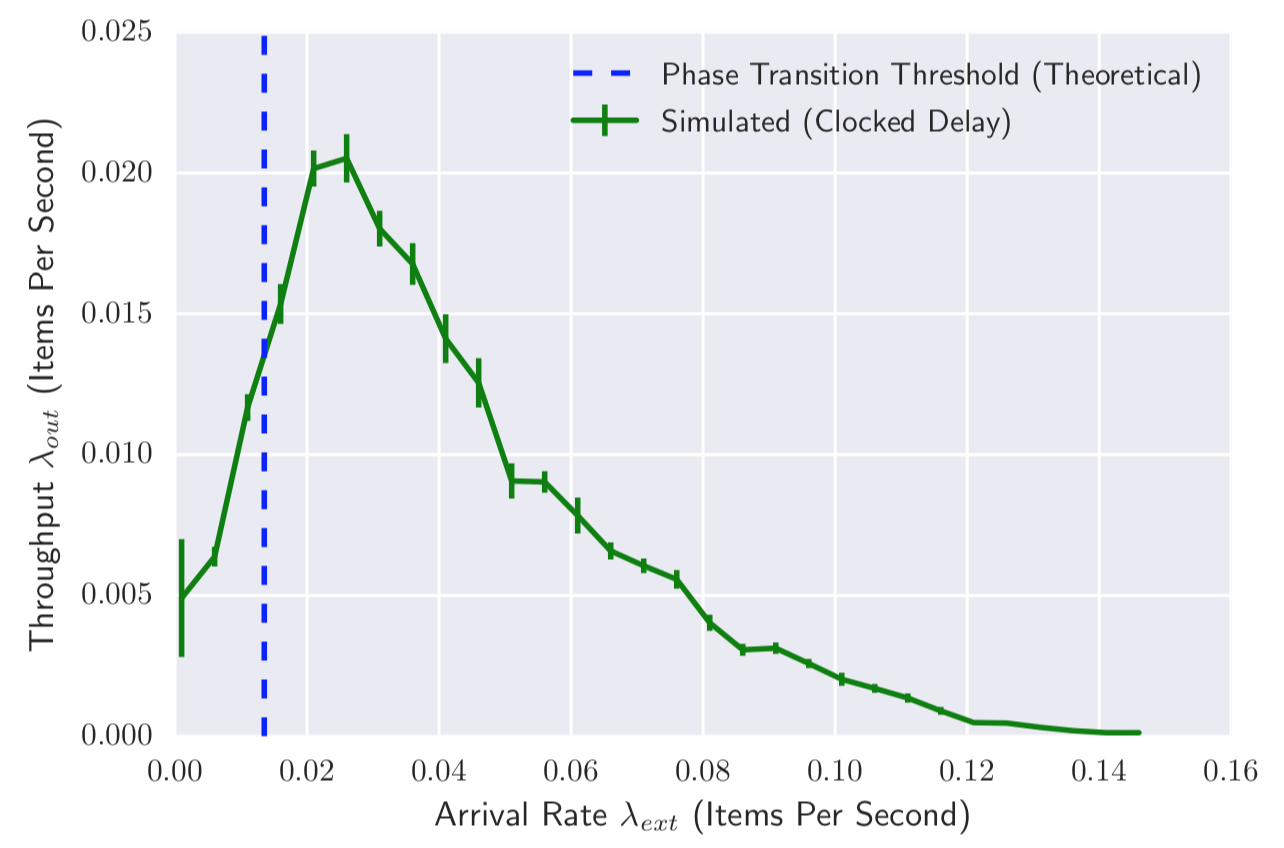
\includegraphics[width=0.75000\textwidth]{assets/phase-transition.png}
\caption[Phase transition in learning: Average learning rate
\(\lambda_{out}\) vs.~arrival rate \(\lambda_{ext}\) in the Leitner
Queue Network with clocked delays, for a session of 500 reviews over 50
items. We set number of decks \(n = 5\), review frequency budget
\(U = 0.1902\), and global item difficulty \(\theta = 0.0077\). The
dashed vertical line is the predicted phase transition threshold under
the mean-recall approximation.]{Phase transition in learning: Average
learning rate \(\lambda_{out}\) vs.~arrival rate \(\lambda_{ext}\) in
the Leitner Queue Network with clocked delays, for a session of 500
reviews over 50 items. We set number of decks \(n = 5\), review
frequency budget \(U = 0.1902\), and global item difficulty
\(\theta = 0.0077\). The dashed vertical line is the predicted phase
transition threshold under the mean-recall
approximation.\footnotemark{}}\label{fig:phase-transition}
\end{figure}
\footnotetext{Figure text taken from paper (Reddy et al. 2016)}

Other minor findings:

\begin{itemize}
\tightlist
\item
  Slightly convex graph of ``Learning rate \(\lambda_{ext}\) vs.
  \(U\)'', for low values of U, meaning increasing returns, at least for
  low values of U. That is, if you decide to study a little more, the
  increase in optimal learning rate \(\lambda_{ext}\) is at least
  proportional to this study budget, or better than linear, which is an
  encouraging for using the system.
\item
  Simulations of the LQN also provided support for the empirical
  observations in the literature for expanding intervals between
  repetitions.
\item
  Exploration through simulation of optimal study strategies, assuming
  non-uniform item difficulty, it was found that easy items should spend
  roughly the same time in each deck, whereas more difficult items
  should spend more time in the lower decks than higher decks.
\end{itemize}

\subsubsection{3: Experimental
Validation}\label{experimental-validation}

\begin{figure}
\centering
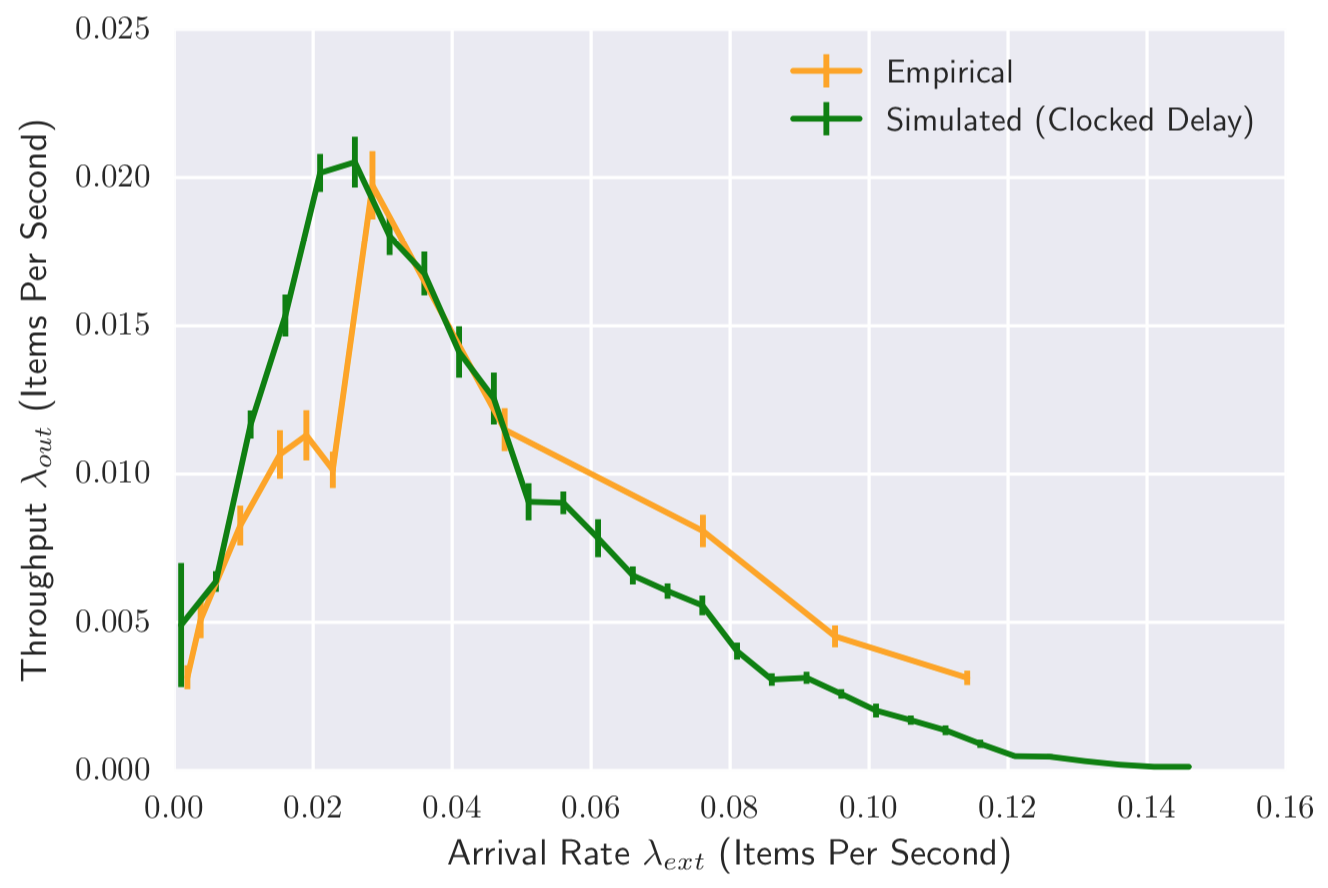
\includegraphics[width=0.75000\textwidth]{assets/verification1.png}
\caption[The exit rate \(\lambda_{out}\) vs.~arrival rate
\(\lambda{ext}\), where number of decks \(n = 5\), review frequency
budget \(U = 0.1902\), and global item difficulty
\(\theta = 0.0077\).]{The exit rate \(\lambda_{out}\) vs.~arrival rate
\(\lambda{ext}\), where number of decks \(n = 5\), review frequency
budget \(U = 0.1902\), and global item difficulty
\(\theta = 0.0077\).\footnotemark{}}\label{fig:verification1fig14}
\end{figure}
\footnotetext{Figure text taken from paper (Reddy et al. 2016)}

\begin{figure}
\centering
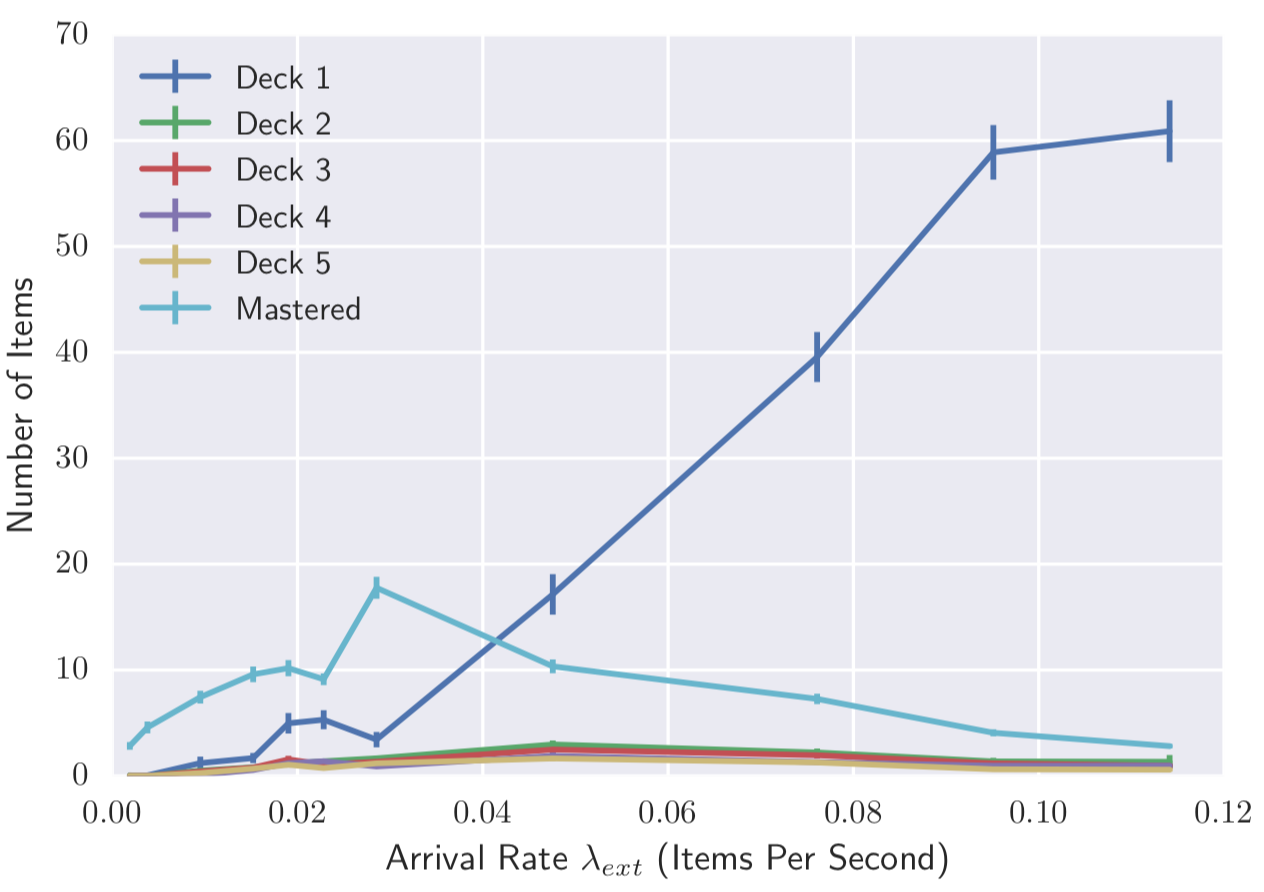
\includegraphics[width=0.75000\textwidth]{assets/verification2.png}
\caption[The number of items that finish in each deck vs.~arrival rate
\(\lambda_{ext}\), where number of decks \(n = 5\), review frequency
budget \(U = 0.1902\), and global item difficulty
\(\theta = 0.0077\).]{The number of items that finish in each deck
vs.~arrival rate \(\lambda_{ext}\), where number of decks \(n = 5\),
review frequency budget \(U = 0.1902\), and global item difficulty
\(\theta = 0.0077\).\footnotemark{}}\label{fig:verification2fig15}
\end{figure}
\footnotetext{Figure text taken from paper (Reddy et al. 2016)}

\begin{figure}
\centering
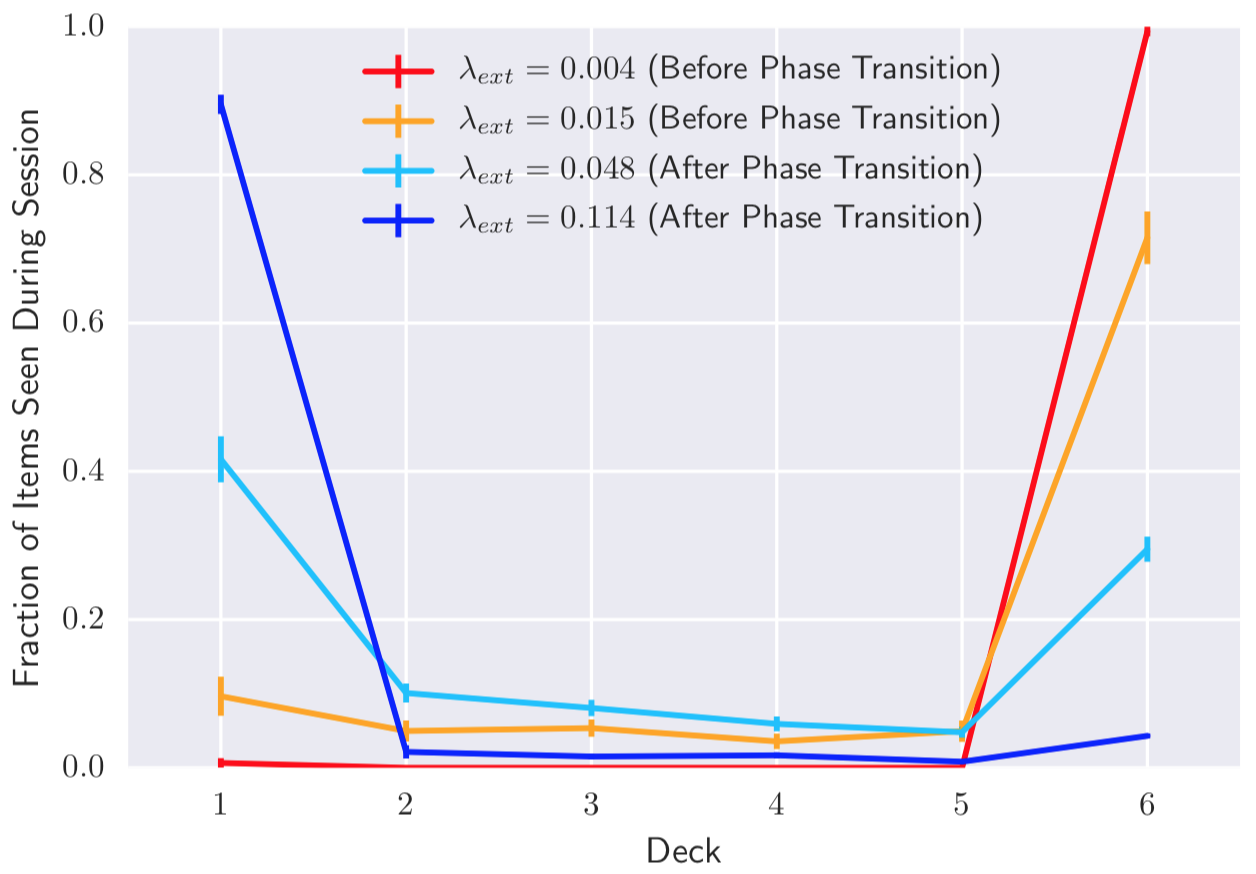
\includegraphics[width=0.75000\textwidth]{assets/verification3.png}
\caption[The fraction of items seen during a session that finish in each
deck for different arrival rates \(\lambda_{ext}\), where number of
decks \(n = 5\), review frequency budget \(U = 0.1902\), and global item
difficulty \(\theta = 0.0077\). Deck 6 refers to the pile of mastered
items.]{The fraction of items seen during a session that finish in each
deck for different arrival rates \(\lambda_{ext}\), where number of
decks \(n = 5\), review frequency budget \(U = 0.1902\), and global item
difficulty \(\theta = 0.0077\). Deck 6 refers to the pile of mastered
items.\footnotemark{}}\label{fig:verification3fig16}
\end{figure}
\footnotetext{Figure text taken from paper (Reddy et al. 2016)}

We see that the phase transition that was found in theoretic analysis
and simulations in the previous sections are found again the in
experimental validation in Fig.~\ref{fig:verification1fig14}.

\begin{quote}
As the arrival rate increases past the optimum, relatively fewer items
are mastered and relatively more items get `stuck' in deck 1.
Intuitively, the user gets overwhelmed by incoming items so that fewer
and fewer items get reviewed often enough to achieve mastery.
Fig.~\ref{fig:verification2fig15} and Fig.~\ref{fig:verification3fig16}
match the behavior suggested by our queueing model: for injection rates
higher than the threshold, the number of items in deck 1 blows up while
the other decks remain stable.
\end{quote}

\subsubsection{Paper Conclusion and Open
Questions}\label{paper-conclusion-and-open-questions}

\begin{quote}
Our work develops the first formal mathematical model for reasoning
about spaced repetition systems that is validated by empirical data and
provides a principled, computationally tractable algorithm for flashcard
review scheduling. Our formalization of the Leitner system suggests the
maximum speed of learning as a natural design metric for spaced
repetition software; using techniques from queueing theory, we derive a
tractable program for calibrating the Leitner system to optimize the
speed of learning. Our queueing framework opens doors to leveraging an
extensive body of work in this area to develop more sophisticated
extensions. To inspire and facilitate future work in this direction, we
release (1) all model and evaluation code, (2) framework code for
carrying out user studies, and (3) the data collected in our Mechanical
Turk study. The data and code for replicating our experiments are
available online at http://siddharth.io/leitnerq.

Our work suggests several directions for further research. The primary
follow-up is to obtain a better understanding of the Leitner Queue
Network; in particular, better approximations with rigorous performance
guarantees. Doing so will allow us to design better control policies,
which ideally could maximize the learning rate in the transient regime.
The latter is critical for designing policies for cramming, a
complementary problem to long-term learning where the number of items to
be learnt is of the same order as the number of reviews. Next, our
queueing model should be modified to incorporate more sophisticated
memory models that more accurately predict the effect of a particular
review schedule on retention. Finally, there is a need for more
extensive experimentation to understand how closely these models of
spaced repetition apply to real-world settings.
\end{quote}

\pagebreak

\section{Solution Discussion}\label{solution-discussion}

\subsection{The Case for Taking Notes}\label{the-case-for-taking-notes}

When the student experiences a moment of understanding in a learning
process (let's call it an ``insight''), there are several good reasons
to write it down:

\begin{itemize}
\tightlist
\item
  The student may simply forget it, so it is worth noting down for
  review later.
\item
  The simple act of writing it down makes it more likely to be
  remembered. Especially in handwriting (May 2014), at least as a first
  iteration, in which case it can be written in computer text later.
\item
  Even if the student have a very good memory, or has been experiencing
  to be doing fine without any note-taking whatsoever, the student may
  have an especially good way of explaining it, which could benefit
  other students in various situations:

  \begin{itemize}
  \tightlist
  \item
    A student that is struggling to understand the same concept could
    benefit from an alternative explanation than that presented in the
    book or lecture.
  \item
    A student who \emph{think} they understand it, but have
    misunderstood a concept partially or completely.
  \item
    A student who also understand it, but in a different way could
    benefit of an alternative explanation, interpretation or mnemonic.
  \item
    Finally, the note could quickly be converted into a flashcard for
    easy quizzing for the exam, and long-term retention after the course
    has ended, if desirable.
  \end{itemize}
\end{itemize}

The good students are most often very willing to help, and by engaging
with the rest of the course, students can act as each other's TAs. It is
also often the case that both the student providing and receiving help
benefits from this interacting.

\subsection{Review Old Class Notes, Books and Video Lectures\ldots{}
Really?}\label{review-old-class-notes-books-and-video-lectures-really}

The study involving the MIT Office of Digital Learning suggests making a
habit out of reviewing (Subirana, Bagiati, and Sarma 2017) (emphasis
added by me):

\begin{quote}
Most notably the key practical advice from our research is that one
should just accept the truth: forgetting is unavoidable. Humans in the
jungle seem to have evolved to best memorize one year or two (so that
only repeated things get memorized), and with time, say 10 years,
mastery reaches its peak. The stronger you memorize something, the
higher you start on the forgetting curve and the longer you have before
reviewing is your only retention option. \textbf{If interested in
learning for life, one should budget time for re-training before
forgetting occurs (and not sooner), even a mild contact with memory
makes it extend its useful life. Make it a habit to review your class
notes, books or even video lectures.}
\end{quote}

If anyone can bring themselves to spend time on reviewing old class
notes, books and video lectures, that is admirable. I believe there is a
better way, which is to produce condensed notes and flashcards (as one
unified material) during learning in collaboration with peers, and then
use \emph{that} to review old classes and courses, falling back on the
original material only if one really want to go in-depth (using deep
linking from notes as suggested).

And finally (Subirana, Bagiati, and Sarma 2017) concludes:

\begin{quote}
First mastery, then retention strategy is what most affects the degree
of learning (many heuristics have been suggested). Plan to use the
skills you know in the following two years (and if not, intensively
re-train). Unless you objectively test your memory, your perception of
accuracy will certainly be wrong and it may be too late when you find
out. Your capacity to memorize does not age, your memories do.
\textbf{Your first job may be the most impactful decision in terms of
how valuable your time at school was (BA, M.Sc, PhD). If related to your
field of study you may be able to use the knowledge and vastly improve
the forgetting threshold. If not, in two years you may lose everything
you got out of it.}
\end{quote}

This exactly part of the problem I wish to solve.

\subsection{Solution Discussion for the Context
Problem}\label{solution-discussion-for-the-context-problem}

We will now revisit the problem of using SRS for conceptual subjects,
but with suggestions for solutions this time.

Spaced repetition is straightforward for very fact-based subjects such
as art history or medicine, where you just need to remember facts, and
the majority of facts are only loosely related to other facts. In
learning languages, word tranlation pairs can be practiced to build a
vocabolary. In all these examples (art history, medicine, languages),
spaced repetition will still be a supplement to actually learning about
e.g.~context of the historical period, the interplay between different
parts of an immune system, or learning language nuance, context and
conversation.

But what about more conceptual subjects such as mathemathics and
physics? The self-taught learner Scott Young\footnote{\href{https://www.scotthyoung.com/}{Scott
  Young} is an author and blogger known for ``The MIT Challenge'', where
  he attempted to learn MIT's 4-year computer science curriculum without
  taking classes in just a year purely by self-study and trying to
  optimize his study techniques (he has also done ``The Year Without
  English'', where he went to learn four languages in one year).} was
initially skeptical of spaced repetition\footnote{https://www.scotthyoung.com/blog/2012/08/05/forgetting-is-good/},
but came around\footnote{https://www.scotthyoung.com/blog/2013/03/31/learning-methods/}
and later posted his thoughts about SRS for conceptual topics\footnote{https://www.scotthyoung.com/blog/2014/11/07/srs-for-concepts}.
He very clearly lays out the big challenge for using SRS in scientific
and technical fields:

\begin{quote}
\begin{enumerate}
\def\labelenumi{\arabic{enumi}.}
\tightlist
\item
  You could try to memorize Newton's 2nd law of motion, F = ma. But that
  is probably one of the least important parts. Having the mathematical
  insight and intuition into knowing what consequences such an equation
  have, what it really means, how it applies to the real world etc., are
  the important things.
\item
  The suggestion is, then, that you don't use SRS to memorize ``facts''
  about physics or math. Instead you use them to prompt questions. So a
  flashcard wouldn't say ``What is Newton's second law?'' but,''Solve
  this set of differential equations.''
\item
  But now the question is what do you solve? Do you solve the same
  question each time? That seems unfair. If I had a complicated
  question, I may not be learning to solve similar questions, but simply
  that the answer is ``x = 7''. We want to understand concepts, not just
  that a particular instance of a problem had a particular answer.
\item
  But if you want variety in your question, you could write a program
  that generates the problem with different numbers randomly.
\item
  This creates a new problem: writing the software to make flashcards
  with randomly generated values. It's not impossible, but it means you
  can no longer just create static content. There is software that does
  this, but it tends to be specialized, meaning it's a lot harder for
  DIY learners who want to learn methods that will work for any subject.
  You need some kind of scripting language to procedurally generate
  problem sets.
\end{enumerate}
\end{quote}

These are extremely good points, and also an opportunity to think out of
the box, and what can be done with a very collaborative and deeply
hierarchical flashcard system. Here are some of the opportunities that
could solve these problems:

\begin{enumerate}
\def\labelenumi{\arabic{enumi}.}
\item
  Since the hierarchy is build into the data structure composing the
  flashcards themselves, you could attach many little bonus questions on
  a single card. You could imagine that a class of students were
  assigned to add some fact about Newton's second law to the card, and
  the validity of these bonus questions could get approved by the
  instructor and/or through peers. For F=ma, this could be:

  \begin{itemize}
  \tightlist
  \item
    For the special case where the acceleration is constant, how does
    the formula integrate to velocity and positions functions v(t) and
    x(t)?
  \item
    What happens when you combine this with Newton's law of universal
    gravity, what does this tell us about falling masses in vacuum?
  \item
    Does this law apply to photons? If not, what law does instead?
  \item
    Etc.
  \end{itemize}
\item
  For conceptual subjects there is typically a natural distinction
  between theory and possible derivation / proof and theory, and
  application. So for every ``theory card'', there could be one of more
  links into ``exercise cards'' and vice versa. This even if you
  remember some equation or concept, you will then stay within context,
  and the next flashcard would be about applying the concept or vice
  versa. I think this staying within the same context for for periods of
  time is one of the key features that are missing from all the
  traditional SRS software.
\item
  Sometimes the context is just two cards: theory/exericse and vice
  versa.
\end{enumerate}

Other times, the context could be a chain of cards, for example in
describing an algorithm or data structure that solves a particular
problem or have a particular set of desired properties. This would
effecively be like going through your notes on the subject, but only
revealing a little part at a time because you want to do active recall
instead of merely re-reading and recognizing information.

\begin{enumerate}
\def\labelenumi{\arabic{enumi}.}
\setcounter{enumi}{3}
\item
  The teacher could contribute with a set of flashcards that are just
  exercises, that are then automatically linked to the student's
  flashcard set both by automatic tag matching and simply by matching
  semester week. By matching keywords from the exercise solutions to
  existing flashards in the student's personal deck and the class'
  collective deck, the student could get hints towards the relevant
  theory without being given the full solution. The spaced repetition
  algorithm could be tuned to show the exercise cards less often than
  concept theory cards (since solving the same exercises more than once
  is generally less useful than solving new exercises).
\item
  Actually go thorugh the effort of making dynamic and interactive
  content and selling this as premium content in an in-app market place.
\end{enumerate}

And interesting problem to be solved is to balance interleaved practice
staying in context. I think this is best solved manually by setting a
particular header level in the hierarchy is a natural unit, meaning that
the system will not move to another subject until all sub-units of the
current unit have been exposed to the user. As an example: perhaps you
want to practice insertion, deletion and search algorithms for a
particular data structure after first recalling the basic structure and
properties of the data structure.

Also, every flashcard should contain a source. It is also important to
emphasize that while some subjects are easier to summarize what
completely into a set of notes, other subjects and endeavors, for
example advanced machine learning more statistics, it is my personal
experience that it is futile to attempt to make a complete set of notes
because you would simply have to almost rewrite text book that you're
reading because it some possible to skip too many details. Instead when
should strive just to save those little important nuggets of information
and not necessarily try to achieve completeness. Making notes in
Flashcards should feel like a net benefit, not a chore. However where
detail is lacking, one should always be able to go o the source, quickly
by use of deep links.

\pagebreak

\section{Product Solution}\label{product-solution}

I envision a collaborative learning platform where students can share
insights on the lectures, reading and other course material, in the form
of ``information chunks'', ``highlights'' or ``take away points'', which
can also be made into flashcards easily. The notes can be
single-sentence note from a book, the web or a lecture, that the student
thought was important enough to remember. Or the notes can be fully
fleshed out and structured notes.

\subsection{Data structure}\label{data-structure}

I think it's crucial to be able to look at the flashcard material either
in hierarchical, organized form where it resembles organized course
notes, where everything is in context. Especially in complex fields such
as science and engineering, there are some kinds of knowledge that lends
itself. The obvious solution to me is therefore notes and flashcards
integrated, with flashcards getting their inherent structure and context
from levels of headers in the notes.

The notes would be simple plain text using a flavor of
Markdown\footnote{Markdown is a very easy to learn markup language that
  was originally made to make it easier to make formatted text for the
  web than using HTML, which involves lots of special tags. For example
  the syntax for writing boldface is
  \texttt{\textless{}string\textgreater{}this\ is\ bold\textless{}/string\textgreater{}}
  in HTML and \texttt{**this\ is\ bold**} in Markdown.} as markup
language to allow flexible formatting, even including citation, math,
footnotes etc. in certain flavors of the language. It is also a
completely open plaintext format, similar to LaTeX. The Markdown syntax
could be extended with a special tag to mark a section of the content as
the answer for a question. The exact syntax isn't important, just the
fact that it would be relatively straight to integrate note-taking with
flashcard creation. This would greatly alleviate the classical problem
of content duplication between notes and flashcards, and most
importantly provide a natural organization and context of the flashcards
for free. All notes are then hierarchical in nature. Every piece of
content will belong to a header on a certain level, for example H1-H6
where H1 is the top level header (title), H2 is subtitle, etc.

This also alleviates the problem of context when reviewing flashcards;
in conceptual subjects (math, physics etc.), it would be relatively
straight forward to stay within the same context or ``on-topic'', by
simply reviewing all flashcards within the same Markdown header level,
either in random or sequential order. When reviewing the flashcard, the
student could even be free to directly navigate to the note if he/she
should choose, although active recall is the best method for long-term
retention, as established earlier.

Finally, it should be possible to make internal links to other notes
within the application.

\subsection{User Interface}\label{user-interface}

It is very important that the application focuses on fast content
creation and the ability to offload snippets of text and thoughts
quickly. It is not possible for me to come up with a perfect UI design
all at once. The UI design process would instead be an elaborate,
iterative process. But I have taken a stab at it, and sketched a few
screens in the app as I imagined them in the first iteration.

\subsubsection{Screen 1: Opening screen}\label{screen-1-opening-screen}

Upon opening the app, the student will be met be a screen that looks
roughly like Fig.~\ref{fig:ui1}. The text input is front and center,
ready to capture any notes, which can be organized immediately by
pressing any recent or starred notes. The rest of the UI is explained in
the figure caption.

\begin{figure}
\centering
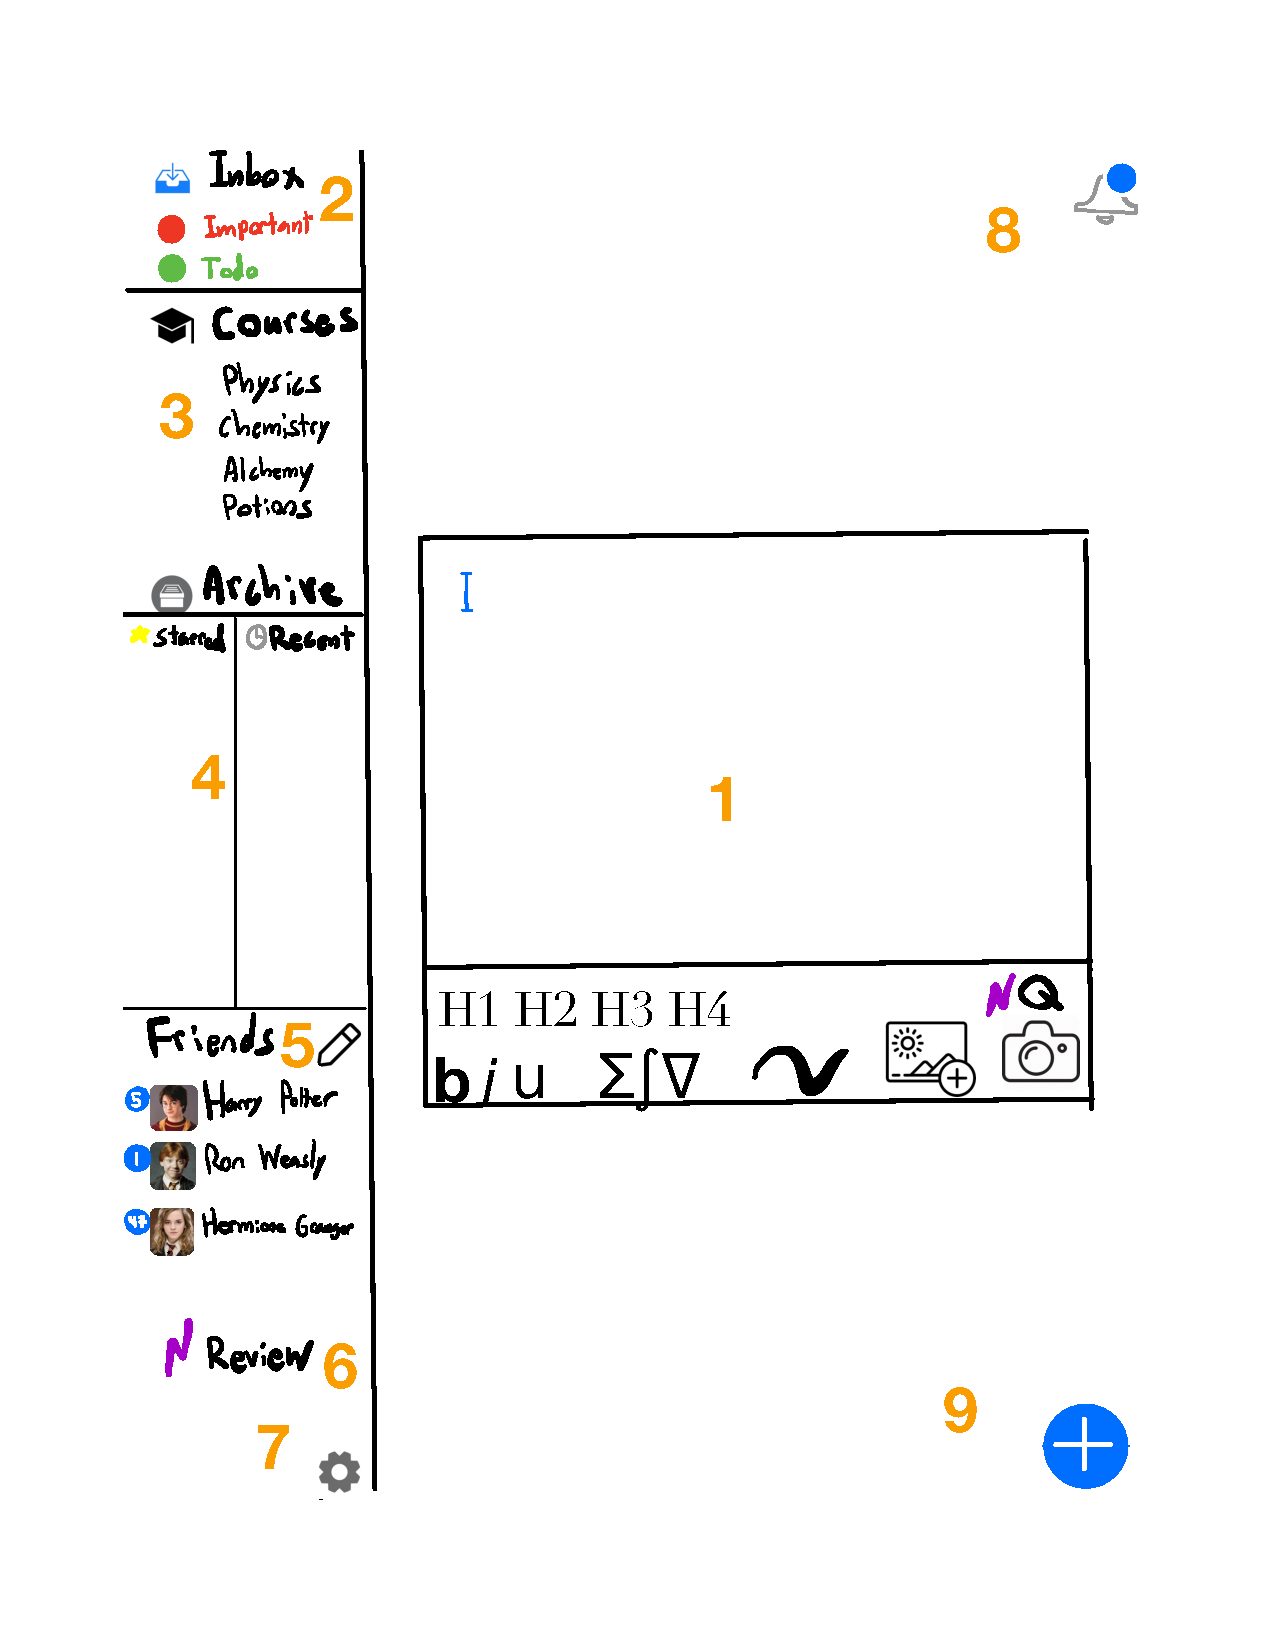
\includegraphics{assets/Flashnotev2-1.pdf}
\caption{1: Note input field, ready to write in startup, 2: Inbox where
notes can be put temporarily, if not organized immediately, and a few
default tags (here Important and Todo), 3: Course list, 4: Starred and
Recent notes for quick navigation and organization of new notes, 5:
Friends list, 6: Review flashcards button, 7: Settings, 8:
Notifications, 9: Quick add note button}\label{fig:ui1}
\end{figure}

\subsubsection{Screen 2: Course screen}\label{screen-2-course-screen}

The course screen (Fig.~\ref{fig:ui2}) shows a given week (or topic)
within a course. It's easy to get an overview of all notes in the
course, and see most upvoted content in the form of notes/flashcards and
take-away points (highlights) and questions from the other students, as
well as extra exercises with solutions.

\begin{figure}
\centering
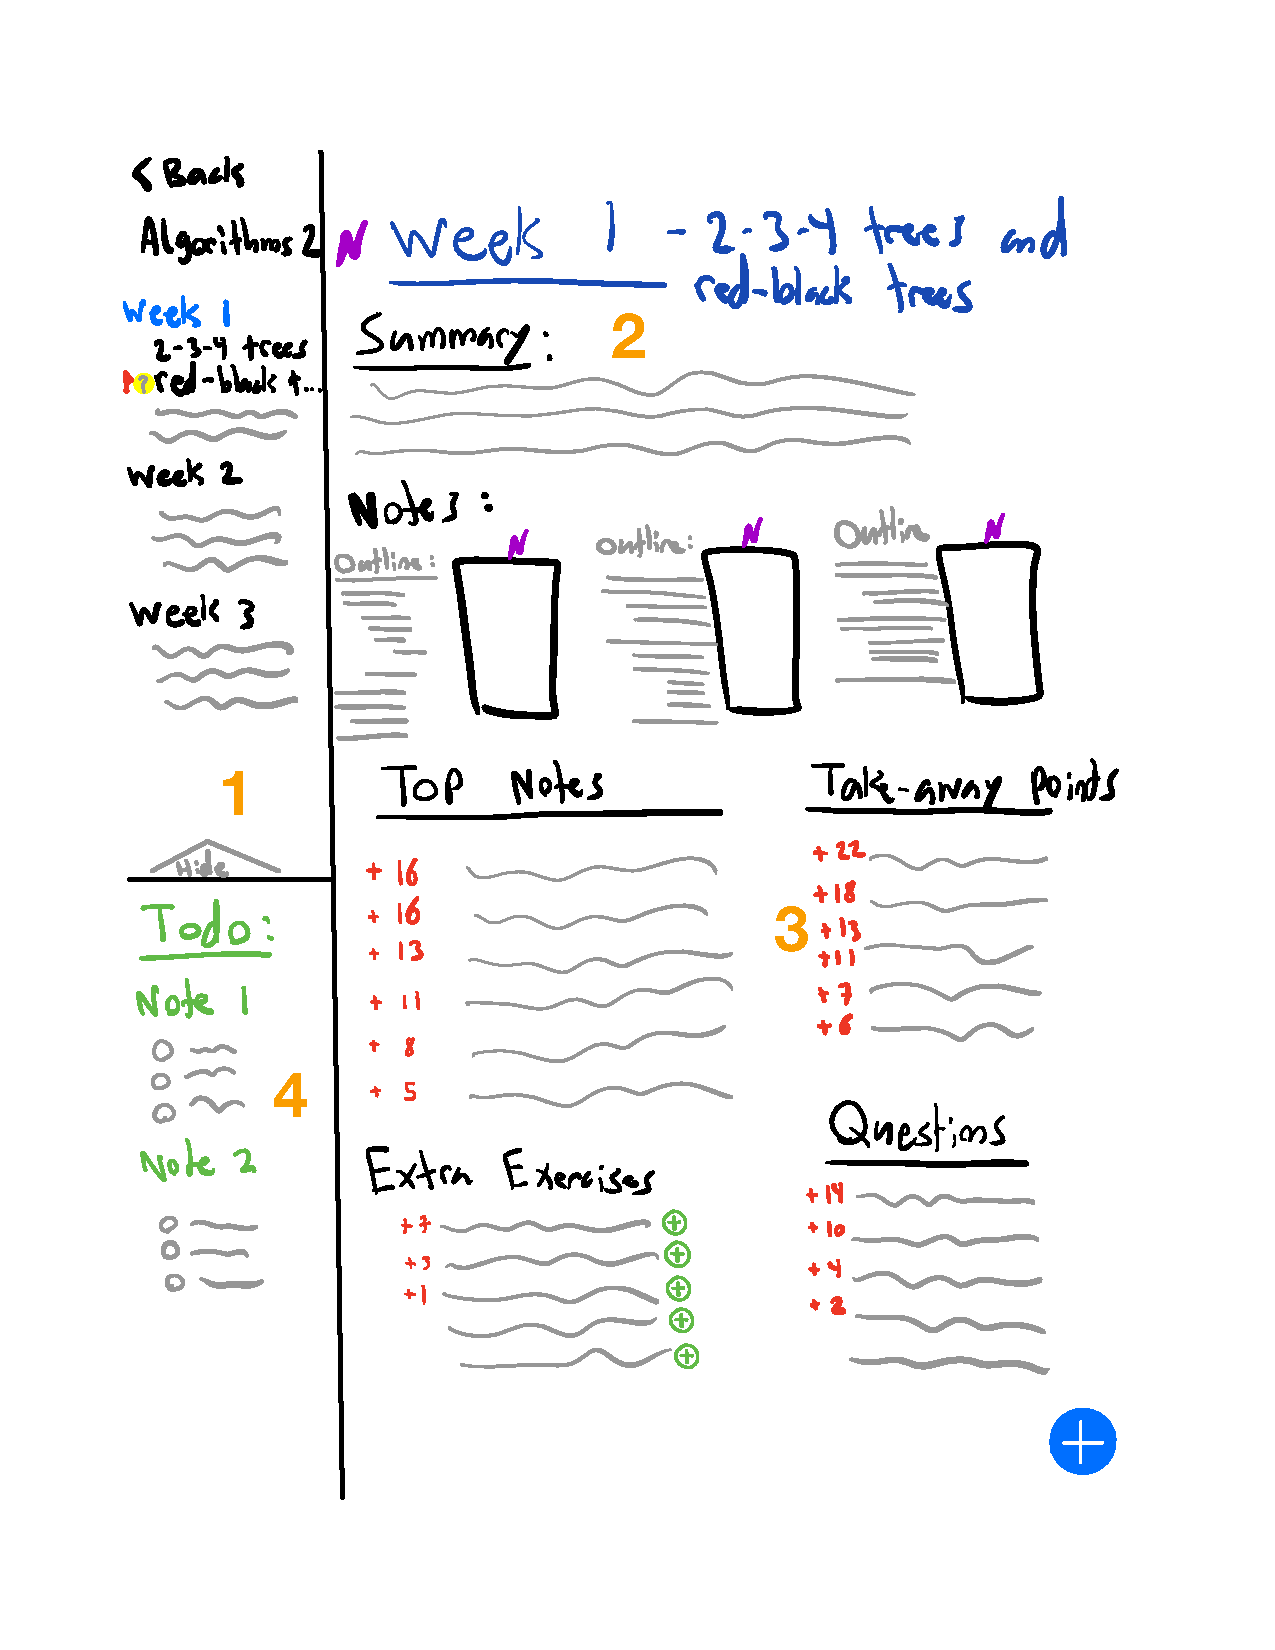
\includegraphics{assets/Flashnotev2-2.pdf}
\caption{1: Course overview and notes list, 2: Course week overview,
including summary and notes with their outlines (i.e.~table of
contents), 3: Most upcated content and questions from the course for
that particular week, 4: Todo list, i.e.~an overview of all notes that
have been tagged as incomplete somewhere, and what is
missing}\label{fig:ui2}
\end{figure}

\subsubsection{Screen 3: Note screen}\label{screen-3-note-screen}

On the note screen (Fig.~\ref{fig:ui3}) we see an example of note
content, including a question and flag from two fellow students. We also
see related notes with own notes and a highly rated note from a peer.
Some content has been marked and paired with questions, forming the
basis of flashcards. The questions can be seen in the right-hand side,
resembling the Cornell method note-taking style.\footnote{https://theconversation.com/whats-the-best-most-effective-way-to-take-notes-41961}

\begin{figure}
\centering
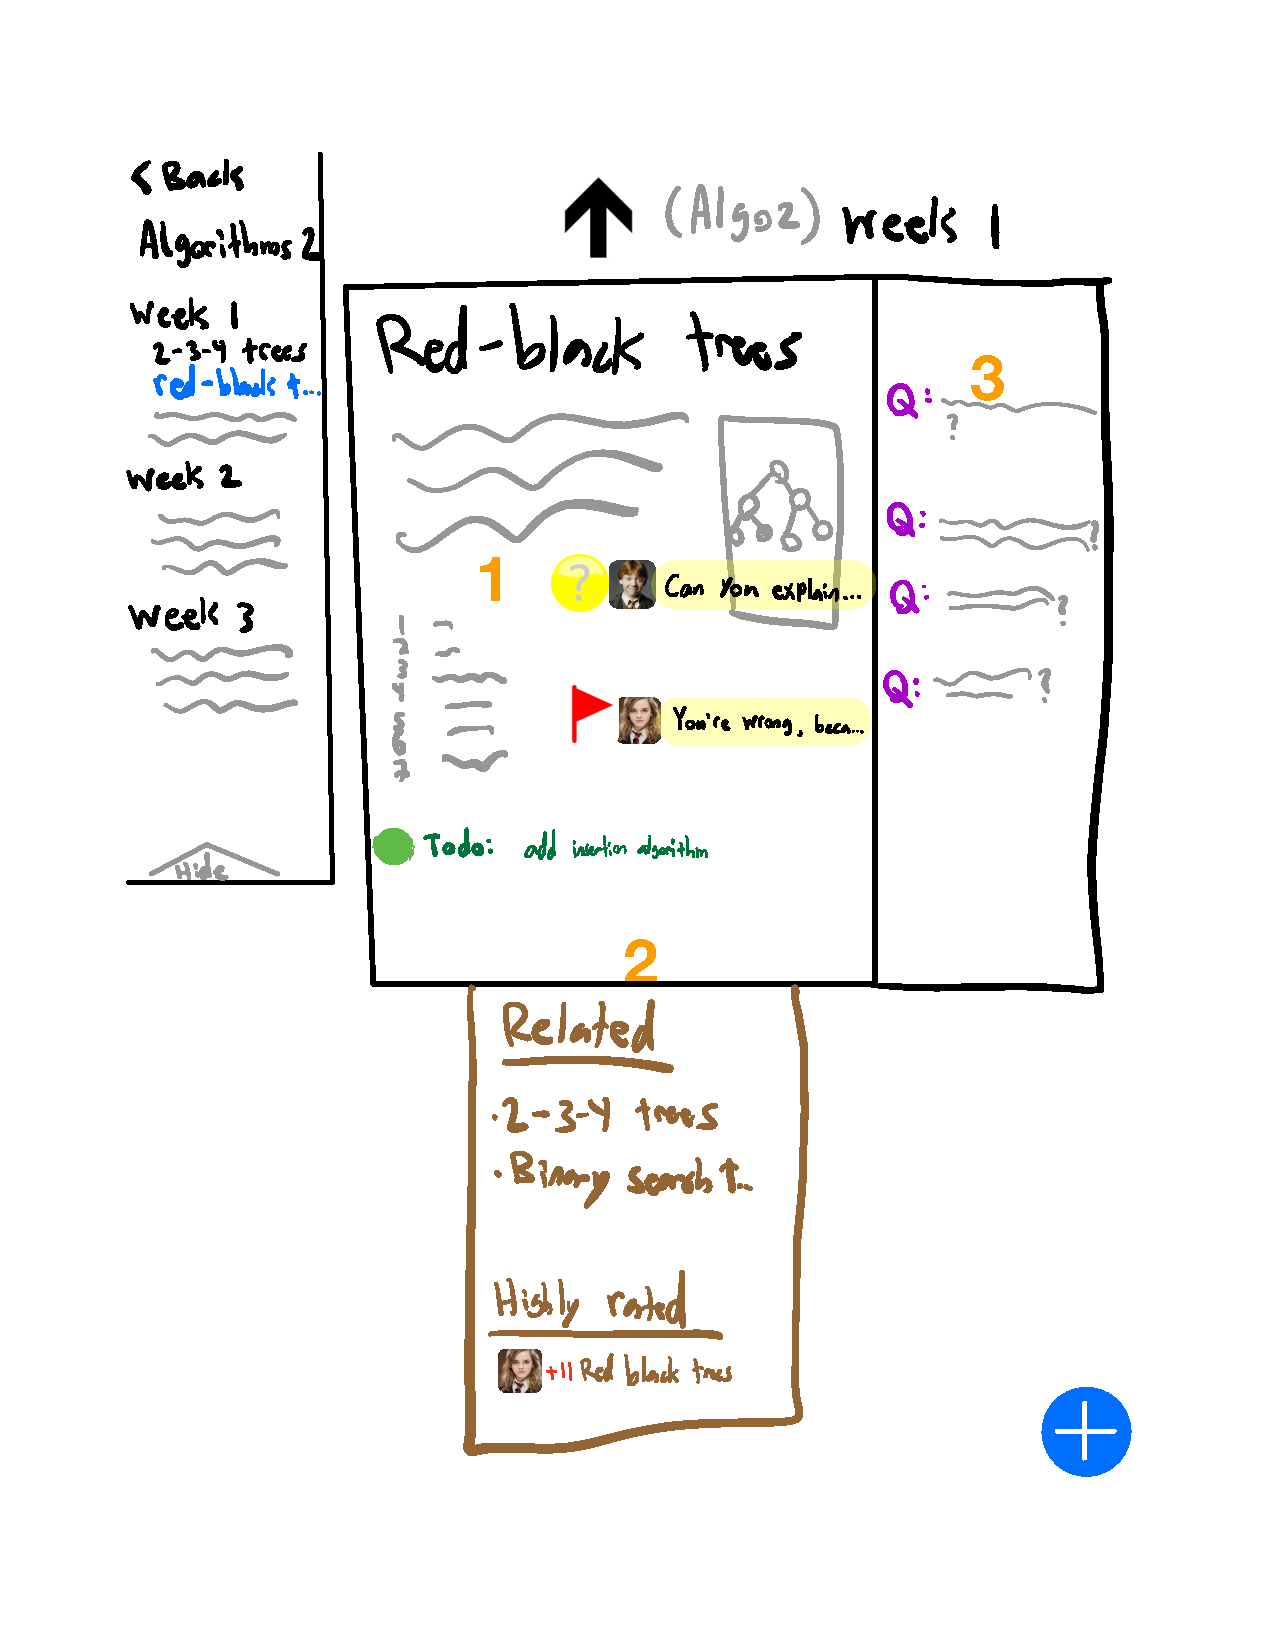
\includegraphics[width=0.90000\textwidth]{assets/Flashnotev2-3.pdf}
\caption{1: Note content 2: Related notes in own library and highly
rated peers3: Questions for content, forming the basis of
flashcards.}\label{fig:ui3}
\end{figure}

\subsection{Key features}\label{key-features}

\begin{itemize}
\tightlist
\item
  \textbf{Note-flashcard hybrid system} - Note-taking system where
  content can be marked and tagged for questions, effectively generating
  flashcards on the notes. We will henceforth call this structure
  ``flashnotes''
\item
  \textbf{Rich collaboration} - Ability to share flashnotes and copy,
  comment, upvote and suggest changes to other people's flashnotes.
\item
  \textbf{Smart scheduling} - Tell the application the date of your
  exams, and it will optimize a review schedule for retention at exam
  date, then switch mode to long-term mastery after that.
\item
  \textbf{Deep linking} - It should be possible (whenever technically
  possible) to create links straight to the source of a flashcard,
  whether that be specific pages in a PDF file or a specific time stamp
  in a YouTube video.
\end{itemize}

\subsection{Bonus Features}\label{bonus-features}

Lastly I will mention some bonus features that would not be present in a
first iteration of the product, but are very exciting possibilities to
consider nonetheless.

\subsubsection{Autotagging for Better Search and Flashcard
Review}\label{autotagging-for-better-search-and-flashcard-review}

There are at least two organizations of notes that makes:

\begin{enumerate}
\def\labelenumi{\arabic{enumi}.}
\tightlist
\item
  Organization according to how it was learning, i.e.~course, week
  number, subject, etc.
\item
  Organization according to how it would be classified in an
  encyclopedia.
\end{enumerate}

It would be possible to crawl through all Wikipedia pages, and construct
a ``knowledge graph skeleton'', i.e.~ignore the content but note how all
the articles link to all the other articles. This could then be
considered as a form of template, whereby arbitrary notes could then be
automatically tagged and classified.

For instance, an note about ``variance'' in statistics could be tagged
with tags \texttt{statistics}, \texttt{standard\ deviation}, and
\texttt{expectation\ value} because concepts are linked to from the
Wikipedia page on variance.

There would be at least two advantages if this could be done
successfully:

\begin{enumerate}
\def\labelenumi{\arabic{enumi}.}
\tightlist
\item
  It would enable even more powerful search in notes, if you want to
  know what notes you have on a particular overall subject, what else
  relates to it. A search field with auto complete suggestions that
  could filter all the notes and generate a word cloud could be a great
  way to explore what you know about a field or concept.
\item
  As we have already discussed, it would likely be beneficial to stay
  within context during flashcard review of complex concept-based
  subjects instead of reviewing cards in completely random order. During
  flashcard review, the note tags from the automatic tagging would
  provide the system with another measure of what concepts are related,
  presumably enchancing the flashcard review experience.
\end{enumerate}

\paragraph{Derived applications: recommendations for courses and
review}\label{derived-applications-recommendations-for-courses-and-review}

Once the student knowledge has be tagged within some kind of objective
tagging framework, it would in principle be possible to offer both
course recommendations based on student interest and ability, as well as
precise recommendations for concepts to review in preparation for
upcoming courses.

\hypertarget{integrated-homework-system}{\subsubsection{Integrated
homework system}\label{integrated-homework-system}}

One could imagine a simple system where students were assigned to for
example:

\begin{itemize}
\tightlist
\item
  Find or invent a cool example where a recently learned concept is
  applied or could be applied.
\item
  As homework, create an assignment or problem for other students to
  solve.
\item
  Peergrade each other's flashcard decks.
\end{itemize}

\subsubsection{Flexible TA employment}\label{flexible-ta-employment}

If a student for any reason display high skills in the course he is
following to such a degree that he can for all practical purposes act as
a TA for his fellow students, why not go the extra step and consider
flexible hire of TAs through the system? There are many practical ways
to handle this, and I have not thought it through yet. It could be that
a student who earns enough ``upvotes'' or ``reputation points'' becomes
eligible for payment as acting TA in the course if she commits to a
certain number of homework assignment grading, or some hours of physical
presence for actually acting as a TA etc. The possibilities are many.
The point is, with a completely transparent system where all notes and
flashcards are shared and discussed, it would be easy to identify the
few very high performing students and actually compensate them if they
wanted to do some extra work.

\subsubsection{Using tags instead of
folders}\label{using-tags-instead-of-folders}

Tags are in general more flexible than folders since an object (here a
note) could belong to multiple tags at the same time, whereas it can
only be located in one folder. The note-taking app Bear\footnote{http://www.bear-writer.com}
launched in 2016 drops the notion of folders entirely and uses tags only
for organization.

\subsubsection{Rich media and flashcard
types}\label{rich-media-and-flashcard-types}

Flashnotes should support audio, video, hand drawing, file attachments
and various structures such as mind maps (for a review of the
\emph{many} card types of FlashCram see (S. Colbran et al. 2014)).

\subsection{Support from learning
theories}\label{support-from-learning-theories}

\subsubsection{Bloom's Taxonomy}\label{blooms-taxonomy}

Bloom's Taxonomy\footnote{For an excellent description and examples of
  use see https://tips.uark.edu/using-blooms-taxonomy/} is a
classification scheme of learning objectives that can help an educator
to design a course. The taxonomy breaks down learning objectives into
six levels of objectives of increasing complexity that builds in one
another, see Fig.~\ref{fig:bloom}

\begin{figure}
\centering
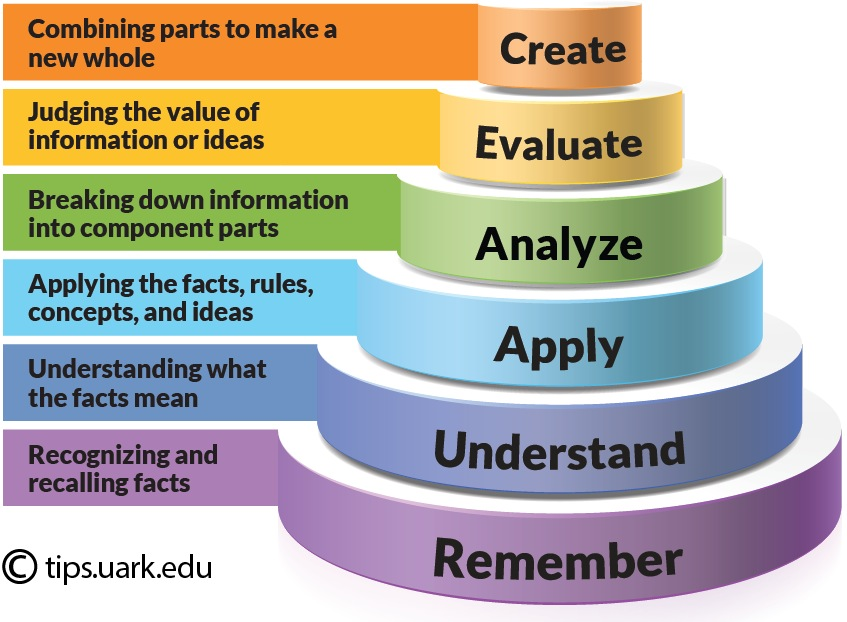
\includegraphics[width=0.65000\textwidth]{assets/Blooms_Taxonomy_pyramid_cake-style-use-with-permission.jpg}
\caption[Bloom's Taxonomy.]{Bloom's
Taxonomy\footnotemark{}.}\label{fig:bloom}
\end{figure}
\footnotetext{For an excellent description and examples of use see
  https://tips.uark.edu/using-blooms-taxonomy/}

The most fundamental level is the bottom ``Remember'', which is the
prerequisite for every learning activity above it. Even if a student has
learned to understand, apply, analyze, evaluate and create, it all still
hinges on the fact that the material can be remembered. One of the
product solution's goals is to facilitate long-term retention, thus it
supports all levels of Bloom's taxonomy \emph{indirectly}. And as we saw
in an earlier section
``\protect\hyperlink{self-testing}{Self-testing}'', self-testing
actually \emph{directly} enhances all levels of learning objectives in
Bloom's Taxonomy.

Furthermore, the suggestions in section
``\protect\hyperlink{integrated-homework-system}{Integrated homework
system}'' easily covers multiple levels of learning objectives in
Bloom's Taxonomy.

\subsubsection{The Case for Collaborative
Co-creation}\label{the-case-for-collaborative-co-creation}

We have seen \href{http://peergrade.io}{Peergrade} take off as a
successful EduTech startup from DTU with finding and support from the
world-class incubator Y Combinator\footnote{https://www.peergrade.io/blog/peergrade-goes-y-combinator/}.
This is with good reason, because the case for aiding students with
collaboration tools and peer-interaction that has only become possible
with technology recently, is strong\footnote{https://www.peergrade.io/pedagogy/}
(Prince 2004) . In their extensive review of digital flashcard tools for
law students, (S. Colbran et al. 2014) discussed this aspect too:

\begin{quote}
For many years academics have been designing learning activities and
assessment tasks enabling students to \emph{learn through making}
{[}5{]} artefacts or engage in \emph{learning by doing.} {[}6{]} These
learning experiences are often informed by constructionism {[}7{]} and
social views of learning. {[}8{]} Put simply, when we discuss and build
an artifact, we learn something about it.

(\ldots{})

Digital students also crave peer review and interaction. Collaboration
is at the heart of learning for them. Learning is a social phenomenon as
well as a cognitive process. {[}28{]} By bouncing ideas off of each
other, students can formulate their own opinions and drive the
discussion themselves. They enjoy learning through discovery and
discussion. {[}29{]} Their collaboration can either be in class, in
person or virtual. {[}30{]} As a result, the professor no longer needs
to be the sole and center point of learning; instead students have many
resources from which to choose. Digital students often set up blogs for
specific issues. They also e-mail and IM each other often (usually in
the middle of class).
\end{quote}

In their review of the online collaborative flashcard platform
FlashCram, more feature similar to the ones I suggest, are mentioned:

\begin{quote}
Users may break and relink sequences of cards. New cards can be easily
added into sequences or as entirely new topics. Old cards may be deleted
or reorganised using a mind mapping construct. Data analytics can
automatically follow the amended sequences providing useful diagnostic
tools associated with student learning.
\end{quote}

What (S. Colbran et al. 2014) sought and ultimately couldn't find (in
2014 at least) sound very close to my exact thoughts:

\begin{quote}
There are a number of digital flashcard websites. A preliminary
evaluation of these sites found no site that meet the authors' immediate
requirements and could evolve as the authors' conception of digital
flashcards developed within a learning model informed by a range of
learning models including some embryonic ideas about connectionism, ie.
representations of knowledge are distributed across a network of
heterogeneous connections - learning being the ability of traverse and
construct one's personal network (albeit shared between a group of
people)
\end{quote}

\subsubsection{Metacognition and
Self-regulation}\label{metacognition-and-self-regulation}

(Huang 2017) writes that ``Reflection is, however, intrinsically linked
to metacognition and self-regulation, where there is ample evidence as
to their importance to learning'', the idea being that ``through
reflection, learners develop their ability to integrate the insights
they gain into their learning/life experience so that they can make
better choices and improve their learning''. This makes sense, and at
DTU we like evaluations a lot already, we do them twice every semester
for every course. This could be another means to have the students
reflect on what we are teaching them, every day.

(S. Colbran et al. 2014) also emphasize that flashcards promotes
critical analysis, synthesis of information and self-reflection:

\begin{quote}
Flashcards are commonly created and shared amongst people seeking to
test their knowledge and memory. The process of construction of the
flashcards promotes learning by doing, critical analysis and synthesis
of information. Revision with flashcards promotes formative assessment
and self-identification of misinterpretations and memory faults, which
may in turn be corrected through self-reflection. Sharing of cards also
affords the opportunity for peer review.
\end{quote}

Being an regular and active creator of notes and flashcards forces you
to take a very active stance in your own learning. The minimum
information principles teach you to ask yourself ``What are the core
ideas of the book I'm reading?''.

\subsubsection{Flashcards Interacting With Various Learning
Theories}\label{flashcards-interacting-with-various-learning-theories}

The display of learning theories developed in the Holistic Approach to
Technology Enhanced Learning (HoTEL) project reminds us of the range of
learning theories available and serves as a nice overview,\footnote{http://hotel-project.eu/content/learning-theories-map-richard-millwood}
see Appendix \ref{sec:hotel}.

(S. Colbran et al. 2014) proceeds to analyze how flashcards are used to
support various learning activities derived from a wide range of
learning theories depicted in the HoTEL framework. They have \emph{a
lot} and I have chosen to quote a subset that made especially good sense
to me:

\begin{quote}
\begin{itemize}
\tightlist
\item
  \textbf{Situated Learning} - Lave and Wenger {[}43{]} - whereby
  knowledge is co-constructed, situated in context and embedded in a
  social and digital environment. This theory sits within the discipline
  of social anthropology. Digital flashcards may be collaboratively
  constructed and shared with peers in a law course via the cloud-based
  FlashCram system.
  \url{https://www.learning-theories.com/situated-learning-theory-lave.html}Situated
  learning ``takes as its focus the relationship between learning and
  the social situation in which it occurs''.{[}1{]}
  \url{https://en.m.wikipedia.org/wiki/Situated_learning}
\item
  \textbf{Constructivism} - Millwood, {[}45{]} von Glaserfeld {[}46{]}
  and Paiget {[}47{]} - the learner is no longer passive, but actively
  constructs knowledge. This theory sits within the disciplines of
  philosophy, cybernetics and anthropology. Digital flashcards can be
  easily incorporated into an assessment design whereby students create,
  document and share knowledge. The proliferation of shared digital
  flashcards available on the Internet on legal topics is testament to
  the ability of digital flashcards to be a tool active construction and
  sharing of knowledge.
\item
  \textbf{Connectivism} - whereby `knowledge is distributed across a
  network of connections to people and information - learning consists
  of the ability to construct and traverse those networks.' {[}49{]}
  This theory sits within the disciplines of Philosophy, Design, and
  Cybernetics. Students may create a network of digital flashcards by
  placing direct links in their digital flashcards to other digital
  resources or may include references to non-digital resources. The aim
  of this task is to make a network of resources, primarily to text,
  audio and video resources. Students may then share links to their
  packs of flashcards.
\item
  \textbf{Expansive learning} - Engestrom {[}50{]} - This theory relates
  to `The learning of new forms of activity as they are created, rather
  than the mastery of putative stable, well-defined, existing knowledge
  and skill'. {[}51{]} The degree of scaffolding provided by academics
  around the creation of digital flashcards may determine the boundaries
  of knowledge captured by digital flashcards. If for example, students
  are asked to develop flashcards on Restitution, the ambiguity of
  boundaries of the topic will enable students to explore the topic more
  excursively than with a very constrained topic.
\end{itemize}

Digital Flashcards align well with the following key concepts from
HoTEL:

\begin{itemize}
\tightlist
\item
  \textbf{Communities of practice} - Lave \& Wenger - Groups of people
  with a common interest learn together through interaction. Exercises
  may be designed to encourage collaborative digital flashcards to
  further a common purpose - examples of such cards include the
  Role-play card, Discussion card, Wiki card, Polling card etc.
\end{itemize}
\end{quote}

\section{Discussion and Reflection}\label{discussion-and-reflection}

\subsection{Measure of Success?}\label{measure-of-success}

When all is said and done, we have still not addressed one of the
central points of the MIT paper (Subirana, Bagiati, and Sarma 2017)
quoted in the introduction on the question ``what do we forget?''

\begin{quote}
On the first question, the vast majority of research focusses on
retention of basic skills for less than a year. No retention of higher
cognitive tasks has been found. For example, only the lower stage of
Bloom's taxonomy {[}61{]} has been analyzed despite it having been
initially introduced over 60 years ago. Surprisingly, the extensive
literature on mastery has been largely ignorant of long-term effects.
The focus has been on short term effects as if the goal was to master
the subject for college education, i.e., to pass the exam and perhaps as
a basis for subsequent courses in a particular subject line, but not to
support a long-term career. I.e., none of the work reviewed so far
addresses the question of what is it we want to measure in terms of
college academics: is it the recall of basic concepts? Is it the ability
to solve problems? Is it the ability to relate the subject to other
forms of knowledge? Is it the ability to find relevant information about
the subject when there is a need for it? Is it the ability to re-learn
the subject? Is it the increase in the size of the cortex? All studies
focus either on exam repetitions or on basic concept recall leaving a
lot of room for speculation of what are the answers to the above
questions. Richardson-Klavehn and Bjork {[}62{]} perform a very
extensive review with about 300 references of the different ways to
measure memory including free recall, cue recall and recognition.
Unfortunately, here we are interested in very long term retention and
all they discuss is short term memory (less than a year) -- however, one
should be able to use the same measure for short term and for long term
experiments.
\end{quote}

These are not trivial questions to answer, and will require years more
research. However the last sentence is reassuring --- all indications so
far are that we \emph{should} be able to use the same measure for short
term and for long term experiments, and that long-term retention also
follow an ``Ebbinghaus forgetting curve''.

\subsection{Speculations on the Workings on Long-term
Memory}\label{speculations-on-the-workings-on-long-term-memory}

(Subirana, Bagiati, and Sarma 2017) concluded:

\begin{quote}
The single and most relevant finding of our research, one we can assert
categorically (pending a full review), is that there is no single
research experiment providing scientific evidence that academic content
learned in college, subsequently-unused, is forgotten at a different
speed than the one predicted by the Ebbinghaus curve: halving retention
every two years.
\end{quote}

Thus Ebbinghaus curve for long-term retention seems like a reasonable
hypothesis until proven otherwise.

However the Ebbinghaus curve is by no means the only possibility on the
workings of long-term memory. (Subirana, Bagiati, and Sarma 2017)
concludes:

\begin{quote}
At the functional level, our review has not found any model of
forgetting that helps predict all the memory retention behaviors
described and the realm of the unanswered covers basic issues such as
whether the mechanism for retention differs depending on the interval.
For example, our review is consistent with three broad operational
models of long-term memory: 1. The first one, which we call the ECM
model (Ebbinghaus Continuity Model) by which the same effects that are
seen short term apply long term with different ``parameters''. This
would explain why things are so easily forgotten and there should be a
call to action in terms of finding optimal re-practice scheduling
alternatives that extend the longevity of relevant learnings. Under this
model, aspects like emotion, embodied cognition or grit simply modulate
an underlying Ebbinghaus-like decay. 2. The second one is that there is
a different type of memory mechanism that applies long-term which does
not follow the Ebbinghaus curve, perhaps one that is more connected to
emotions and less to short-term memory. Just like we have nuclear,
gravitational and electric forces, each of which applies at a different
level, we may have a ``one-year'' mechanism that applies to attain
mastery but that there is a second one that applies in the long term.
This second view may be consistent with some of the differences found in
memory performance across experiments. The human brain may have adapted
to a dual memory system, a four-season one-shot mastery-optimized cycle
(that explains the perverseness of the short-term memory research and
curriculum planning) and a longer-term memory system that operates under
different norms retention-based where loyalty and group values
predominate and where mastery is not as important. 3. A third one would
be that memory is alive, it behaves as a constantly changing organism
that has a life of its own. It operates by guessing what we need from it
and selectively forgets and evolves suggesting people forget what they
learn in college because they sense it's useless beyond an exam, not
because Ebbinghaus dictates it.
\end{quote}

It will be very exciting to follow the research in this area as we
hopefully get closer the which if the models above best reflect human
memory. The scope of the SRS learning platform proposed in this report
is to address the retention problem as good as possible based on the
abundant up-to-1-year-retention-research, and assume that the effect
will reflect into the long term (as preliminary research could
indicate). Then adjustments can be made if new research on specifically
long-term retention comes out with relevant findings.

\subsection{Why Is Spaced Repetition Not Used in
School?}\label{why-is-spaced-repetition-not-used-in-school}

(Dunlosky et al. 2013) gives two reasons why students don't use more
efficient study techniques:

\begin{enumerate}
\def\labelenumi{\arabic{enumi}.}
\tightlist
\item
  The teachers themselves are not schooled in them.
\item
  The educational system puts emphasis on teaching students
  critical-thinking skills and delivering content. ``Less time is spent
  on teaching them how to learn. The result can be that students that do
  well in their early years, when learning is closely supervised, may
  struggle once they are expected to regulate their own learning in high
  school or college.''
\end{enumerate}

But why don't the universities push spaced repetition more? (Kang 2016)
offers two explanations:

\begin{quote}
Probably (at least) two major obstacles impede greater implementation of
spaced practice in education.

When deciding on what instructional techniques to use (and when to use
them), many teachers default to familiar methods (e.g., how they
themselves were taught; Lortie, 1975) or rely on their intuitions, both
less than ideal: Our intuitions about learning can sometimes be plain
wrong, and it would be a waste to overlook the growing evidence base
regarding the effectiveness of various teaching or learning strategies.
A possible solution is for teacher preparation to increase its focus on
the science of learning (e.g., how the human mind learns, what factors
influence learning, learning strategies, and their relative efficacy).

The second major hurdle is conventional instructional practice, which
typically favors massed practice. Teaching materials and aids (e.g.,
textbooks, worksheets) are usually organized in a modular way, which
makes massed practice convenient. After presenting a new topic in class,
teachers commonly give students practice with the topic via a homework
assignment. But aside from that block of practice shortly after the
introduction of a topic, no further practice usually follows, until a
review session prior to a major exam. What this means for teachers
deciding to incorporate spaced practice in their classrooms is that some
planning is required. Complete overhaul of teaching practice may be
difficult, but modifying homework assignments is probably an achievable
target. The classroom-based studies described earlier (Rohrer et al.,
2014; Rohrer et al., 2015) show how a small change in homework
assignments---switching from having the practice problems in a given
assignment on just one topic, to having a mix of problems pertaining to
various topics appearing in each assignment---can dramatically improve
mathematics learning.
\end{quote}

Carolyn Vash put it more bluntly back in 1989 (Vash 1989, 1547):

\begin{quote}
Education policy setters know perfectly well that
\protect\hyperlink{spaced-practice}{spaced practice} works better
{[}than massed practice{]}. They don't care. It isn't tidy. It doesn't
let teachers teach a unit and dust off their hands quickly with a nice
sense of `Well, that's done.'
\end{quote}

I can see the historical reasons for why there has been too much inertia
in the system a change towards practices recommendations by learning
researchers. But I believe this is something we should change now. We
can start small; some recommendations such as reordering the homework
assignments should be easy to implement as a start. DTU have been
willing to roll out Peergrade at DTU on a relatively large scale already
- which is fantastic - but I think we should do more in the areas of
interleaving and spaced repetition.

\begin{quote}
At the end of the 19th century, William James (1899) exhorted teachers
to encourage spaced practice in their students:

\emph{You now see why ``cramming'' must be so poor a mode of study.
Cramming seeks to stamp things in by intense application immediately
before the ordeal. But a thing thus learned can form but few
associations. On the other hand, the same thing recurring on different
days, in different contexts, read, recited on, referred to again and
again, related to other things and reviewed, gets well wrought into the
mental structure. This is the reason why you should enforce on your
pupils habits of continuous application. (p.~129)}

\textbf{The advice given over a 100 years ago is still completely
applicable today, bolstered by the added weight of strong scientific
evidence. My hope is that educators will embrace creative ways to foster
spaced practice in and outside the classroom for the benefit of their
students' learning.} (Kang 2016)
\end{quote}

\section{Conclusion}\label{conclusion}

Research on study techniques and memory research are strongly supporting
systems of \emph{spaced repetition}. A \emph{collaborative} spaced
repetition system has been framed within various learning theories. I
have made the case for why I note-taking is beneficial, and why trying
to memorize anything is useful in the first place.

Some traditional problems with flashcards has been highlighted, most
notably the problem of flashcards is their inherent tendency to become
isolated facts instead of an interconnected web of knowledge. This
problem is especially pronounced in STEM subjects. Solutions to this
problem has been proposed in the form of a hybrid note-taking-flashcard
system where understandings and insights from a course can be shared
among course participants, who simultaneously can begin spread out their
exam preparation in the whole semester, as well as having the means to
remember the course material beyond the exam date.

A review of recent progress in optimizing spaced repetition scheduling
for digital flashcards has also been reviews. We have gone through a
discussion of the areas of still lacking research, mostly related to the
workings of long-term memory (meaning timescales of more than a year),
as well as possible reasons to why neither students nor institutions
seems to be interested in spaced repetition and interleaving, despite
the strong evidence. Finally, the specifics of the learning platform
proposal have been presented, including data structure, key features and
exciting possibilities that presents themselves as suggestions for
unique bonus features.

We will end on a 30-year old quote that still rings true today:

\begin{quote}
\textbf{Despite over a century of research findings demonstrating the
spacing effect, however, it does not have widespread application in the
classroom. The spacing effect is ``a case study in the failure to apply
the results of psychological research''} (Dempster 1988)
\end{quote}

\newpage

\section{Further Reading}\label{further-reading}

The following are the sources I found most useful and/or interesting
during my research, and are consequently the most heavily cited in the
report. I highly recommend reading any and all of them:

\begin{itemize}
\tightlist
\item
  (Branwen 2009) Already an ``internet classic'', a huge article
  focusing on spaced repetition and flashcards with \emph{many} research
  paper citations as well as practical advice.
\item
  (Subirana, Bagiati, and Sarma 2017) - From MIT Office of Digital
  Learning, an excellent review of the state of memory research based on
  a broad survey of hundreds of papers, especially lamenting the lack of
  memory research on long-term memory, i.e.~time scales of more than a
  year.
\item
  (Kang 2016) - From Dartmouth College Cognition and Education Lab, a
  very good overview of both self-testing, spaced practice, spaced
  repetition and interleaving, especially studies done on real-world
  class rooms, in particular STEM subjects.
\item
  (Reddy et al. 2016) - The most technical of the papers and very
  clearly written. It focuses on the mathematical modeling of human
  memory, theoretical analysis, verification of memory models on big
  open datasets using maximum likelihood methods, application of queue
  theory to a Leitner-type spaced repetition system (dubbed a ``Leitner
  Queue Network''), verification of this Leitner Queue Network of by
  simulations, and finally usage of Amazon Mechanical Turk to for
  verification of the Leitner Queue Network.
\end{itemize}

\newpage

\section{References}\label{references}

\setlength{\parindent}{0pt} \setlength{\parskip}{6pt plus 2pt minus 1pt}

\hypertarget{refs}{}
\hypertarget{ref-Averell2011}{}
Averell, Lee, and Andrew Heathcote. 2011. ``The form of the forgetting
curve and the fate of memories.'' \emph{Journal of Mathematical
Psychology} 55 (1): 25--35.
doi:\href{https://doi.org/10.1016/j.jmp.2010.08.009}{10.1016/j.jmp.2010.08.009}.

\hypertarget{ref-Bacon2006}{}
Bacon, Donald R., and Kim A. Stewart. 2006. ``How Fast Do Students
Forget What They Learn in Consumer Behavior? A Longitudinal Study.''
\emph{Journal of Marketing Education} 28 (3): 181--92.
doi:\href{https://doi.org/10.1177/0273475306291463}{10.1177/0273475306291463}.

\hypertarget{ref-Gwern2009}{}
Branwen, Gwern. 2009. ``Spaced repetition.''
doi:\href{https://doi.org/10.1016/j.juro.2006.11.074.}{10.1016/j.juro.2006.11.074.}

\hypertarget{ref-Colbran2014}{}
Colbran, Stephen, Stephen Colbran, Anthony Gilding, and Samuel Colbran.
2014. ``The role of digital flashcards in legal education: theory and
potential.'' \emph{European Journal of Law and Technology} 5 (1).
\url{http://ejlt.org/article/view/320/424}.

\hypertarget{ref-Dempster1988}{}
Dempster, Frank N. 1988. ``The spacing effect: A case study in the
failure to apply the results of psychological research.'' \emph{American
Psychologist} 43 (8): 627--34.
doi:\href{https://doi.org/10.1037/0003-066X.43.8.627}{10.1037/0003-066X.43.8.627}.

\hypertarget{ref-Dunlosky2013}{}
Dunlosky, John, Katherine A. Rawson, Elizabeth J. Marsh, Mitchell J.
Nathan, and Daniel T. Willingham. 2013. ``What Works, What Doesn't.''
\emph{Scientific American Mind} 24 (4). Nature Publishing Group: 46--53.
doi:\href{https://doi.org/10.1038/scientificamericanmind0913-46}{10.1038/scientificamericanmind0913-46}.

\hypertarget{ref-Wired2012}{}
``Everything You Thought You Knew About Learning Is Wrong.'' 2012.
\url{https://www.wired.com/2012/01/everything-about-learning/}.

\hypertarget{ref-Forrin2017}{}
Forrin, Noah D., and Colin M. MacLeod. 2017. ``This time it's personal:
the memory benefit of hearing oneself.'' \emph{Memory}, October.
Routledge, 1--6.
doi:\href{https://doi.org/10.1080/09658211.2017.1383434}{10.1080/09658211.2017.1383434}.

\hypertarget{ref-Huang2017}{}
Huang, Li-Shih. 2017. ``Three Ideas for Implementing Learner
Reflection.''
\href{https://www.facultyfocus.com/articles/teaching-and-learning/three-ideas-implementing-learner-reflection/?\%7B/_\%7Dhsenc=p2ANqtz-8eLpOBN9g13h\%7B/_\%7DhUhYjq9HTN1ybSf45tZ598vas2gqQzmKof51lUd3G4zEvGpYzfoiOhcygk6ZEHDlefG1\%7B/_\%7DTi70nBxxtg\%7B/\#\%7Dcontinued}{https://www.facultyfocus.com/articles/teaching-and-learning/three-ideas-implementing-learner-reflection/?\{\textbackslash{}\_\}hsenc=p2ANqtz-8eLpOBN9g13h\{\textbackslash{}\_\}hUhYjq9HTN1ybSf45tZ598vas2gqQzmKof51lUd3G4zEvGpYzfoiOhcygk6ZEHDlefG1\{\textbackslash{}\_\}Ti70nBxxtg\{\textbackslash{}\#\}continued}.

\hypertarget{ref-Kang2016}{}
Kang, Sean H. K. 2016. ``Spaced Repetition Promotes Efficient and
Effective Learning.'' \emph{Policy Insights from the Behavioral and
Brain Sciences} 3 (1): 12--19.
doi:\href{https://doi.org/10.1177/2372732215624708}{10.1177/2372732215624708}.

\hypertarget{ref-May2014}{}
May, Cindi. 2014. ``A Learning Secret: Don't Take Notes with a Laptop -
Scientific American.''
\url{https://www.scientificamerican.com/article/a-learning-secret-don-t-take-notes-with-a-laptop/}.

\hypertarget{ref-Murre2015}{}
Murre, Jaap M.J., and Joeri Dros. 2015. ``Replication and analysis of
Ebbinghaus' forgetting curve.'' \emph{PLoS ONE} 10 (7): 1--23.
doi:\href{https://doi.org/10.1371/journal.pone.0120644}{10.1371/journal.pone.0120644}.

\hypertarget{ref-Prince2004}{}
Prince, M. 2004. ``Does active learning work? A review of the
research.'' \emph{Journal of Engineering Education} 93 (3): 223--32.
doi:\href{https://doi.org/10.1002/j.2168-9830.2004.tb00809.x}{10.1002/j.2168-9830.2004.tb00809.x}.

\hypertarget{ref-Reddy2016}{}
Reddy, Siddharth, Igor Labutov, Siddhartha Banerjee, and Thorsten
Joachims. 2016. ``Unbounded Human Learning: Optimal Scheduling for
Spaced Repetition.''
doi:\href{https://doi.org/10.1145/2939672.2939850}{10.1145/2939672.2939850}.

\hypertarget{ref-Reddy2017}{}
Reddy, Siddharth, Sergey Levine, and Anca Dragan. n.d. ``Accelerating
Human Learning with Deep Reinforcement Learning.''

\hypertarget{ref-Richards2017}{}
Richards, Blake A, and Paul W Frankland. 2017. ``The Persistence and
Transience of Memory.'' \emph{Neuron} 94 (6). Elsevier: 1071--84.
doi:\href{https://doi.org/10.1016/j.neuron.2017.04.037}{10.1016/j.neuron.2017.04.037}.

\hypertarget{ref-Subirana2017}{}
Subirana, Brian, Aikaterini Bagiati, and Sanjay Sarma. 2017. ``on the
Forgetting of College Academics : At ` Ebbinghaus Speed '?'' no. 068:
1--12.

\hypertarget{ref-Tereda2017}{}
Terada, Youki. 2017. ``Why Students Forget---and What You Can Do About
It.''
\url{https://www.edutopia.org/article/why-students-forget-and-what-you-can-do-about-it}.

\hypertarget{ref-Vacha1993}{}
Vacha, E. F., and M. J. McBride. 1993. ``Cramming: A barrier to student
success, a way to beat the system or an effective learning strategy?''
\emph{College Student Journal} 27 (1): 2--11.

\hypertarget{ref-Vash1989}{}
Vash, Carolyn L. 1989. ``The spacing effect: A case study in the failure
to apply the results of psychological research.'' \emph{American
Psychologist} 44 (12): 1547--7.
doi:\href{https://doi.org/10.1037//0003-066X.44.12.1547.a}{10.1037//0003-066X.44.12.1547.a}.

\newpage

\appendix

\section{Appendix}\label{appendix}

\subsection{Front Page Logo
Explanation}\label{front-page-logo-explanation}

\begin{figure}
\centering
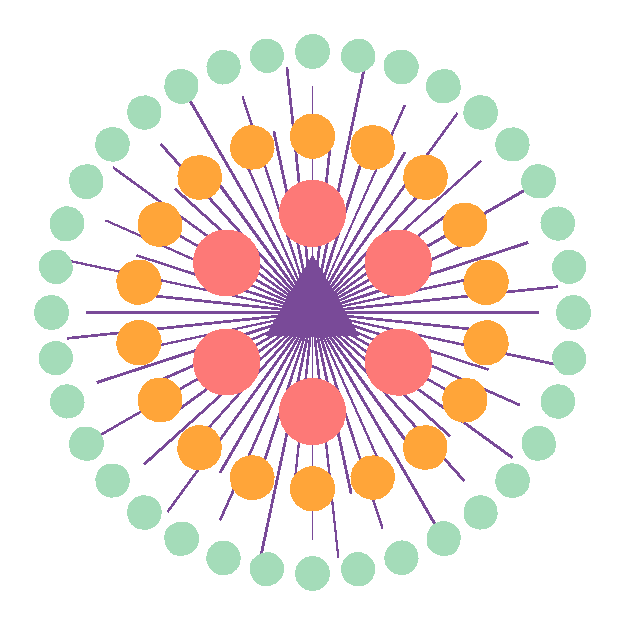
\includegraphics{assets/logo.pdf}
\caption{Front page logo.}
\end{figure}

\begin{itemize}
\tightlist
\item
  \textbf{The purple triangle} in the middle symbolizes the individual
  student who is learning.
\item
  \textbf{The red inner circle} symbolizes the student's immediate
  \emph{friend circle} who is participating in the same learning course
  / learning activity.
\item
  \textbf{The orange middle circle} symbolizes \emph{all} the students
  who is participating in the same learning course / learning activity.
\item
  \textbf{The green outer circle} symbolizes the rest of the world.
\item
  \textbf{The purple rays} emanating from the self in the middle
  symbolizes thought activity and understanding from the student.
\end{itemize}

The whole symbol is meant to symbolize how every single student can
affect and collaborate with the whole course, and even the whole world
during their learning activities, instead of mostly interacting with
their closest friends.

\newpage

\subsection{Early prototype}\label{sec:prototype}

The following prototype developed during the course was inspired by
Microsoft OneNote for interface and organization features, and then
added flashcard capabilities on top.

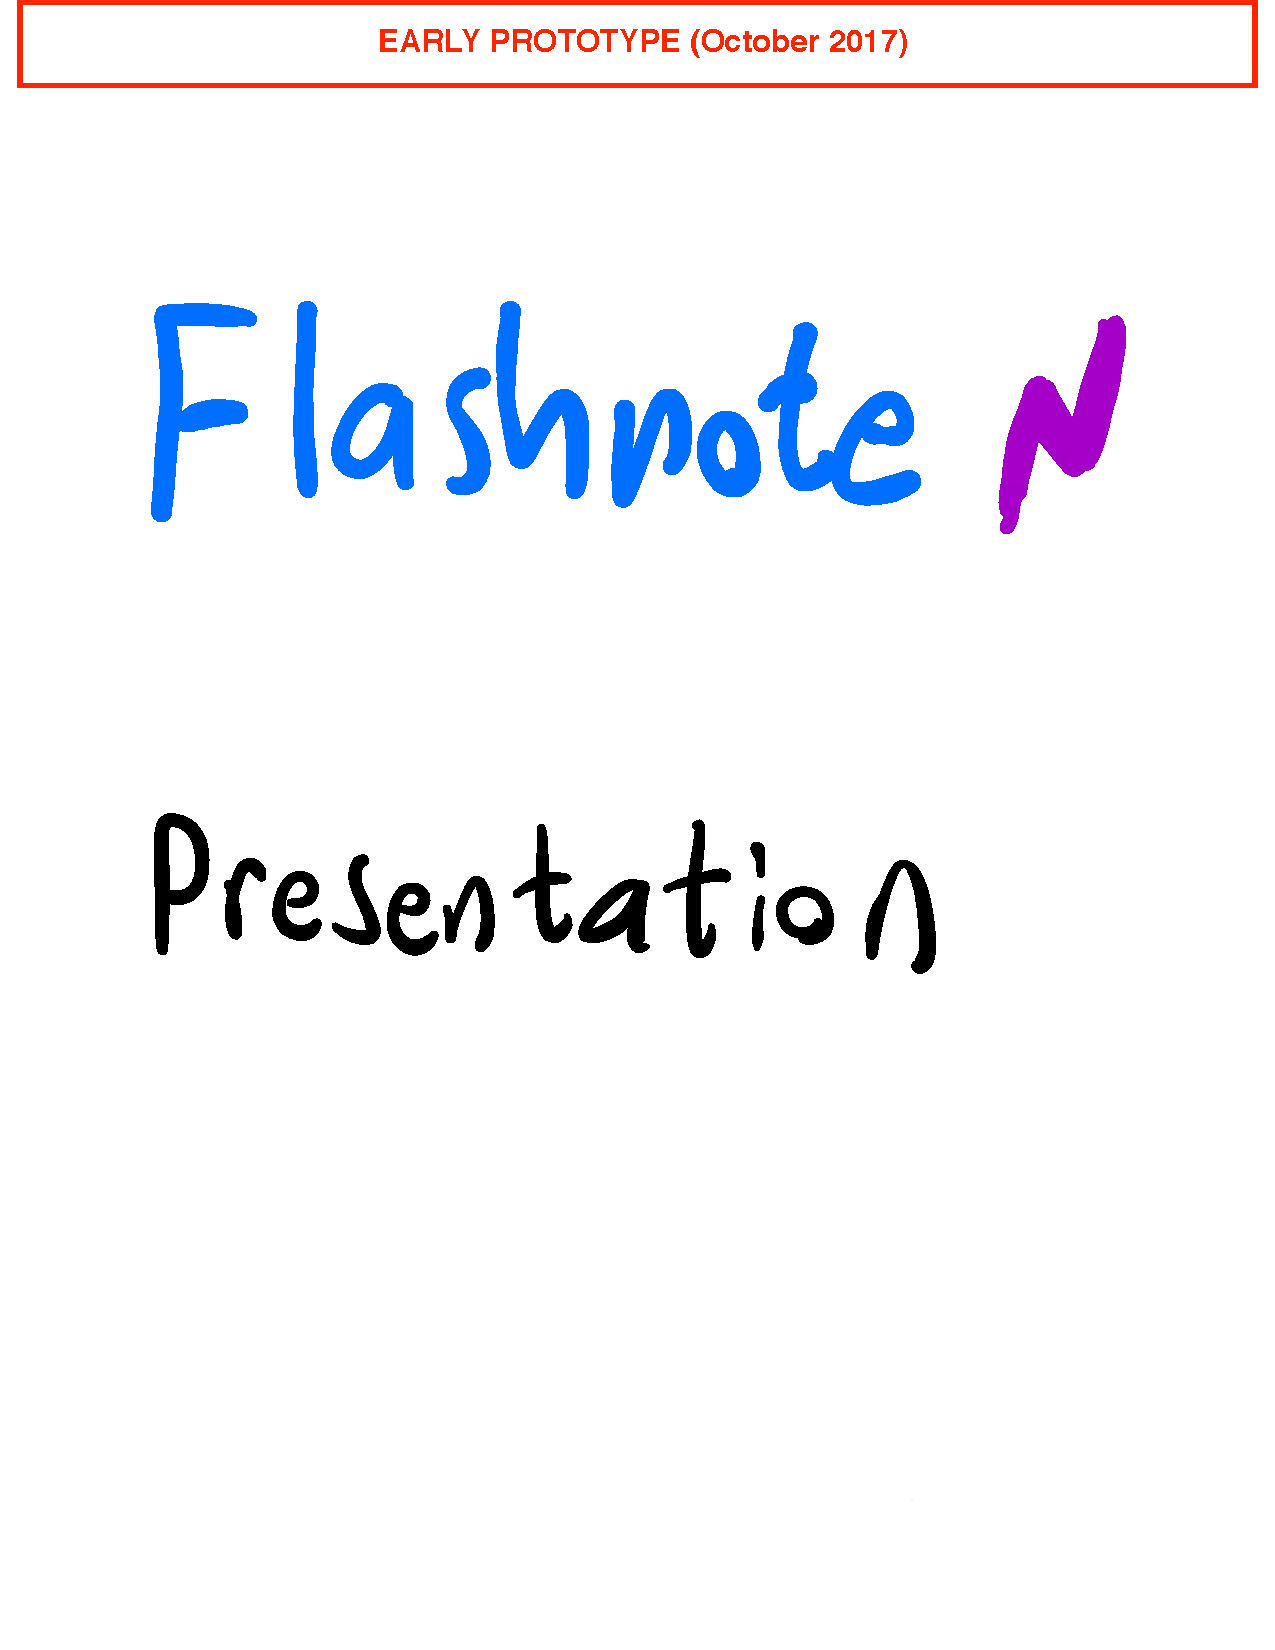
\includepdf[pages=-]{assets/FlashnotePresentationFlatten.pdf}

\newpage

\subsection{Spaced and Interleaved Practice in the
Classroom}\label{sec:classroom}

The following is a quoted section of paper (Kang 2016), emphasis added
by me:

\begin{quote}
Although most studies on spaced or interleaved practice have been
conducted in laboratory settings (for better control over extraneous
variables), students in actual classrooms can benefit from instructors
using these learning strategies (e.g., Carpenter et al., 2009; Sobel,
Cepeda, \& Kapler, 2011). A few studies were conducted not only in
real-world educational settings but also in the context of a regular
curriculum (i.e., instructional manipulation on course content).

In one classroom-based study, the mathematics homework assignments for
seventh-grade students were manipulated across 9 weeks (Rohrer, Dedrick,
\& Burgess, 2014). Ten mathematics assignments were given out over that
period, each consisting of 12 practice problems. For topics assigned to
blocked practice, all 12 problems in a single assignment would pertain
to that one topic (and no other assignment would feature that kind of
problem). For topics assigned to interleaved practice, only the first
four problems in the assignment would belong to the current topic; the
other eight problems in the assignment would cover previous topics;
also, the remaining eight practice problems pertaining to the current
topic (of the first four problems) would be distributed across future
assignments. That is, the total number of practice problems devoted to
each topic was equal across the blocked and interleaved conditions (12
practice problems per topic). The only difference was whether all 12
problems on a given topic were completed in one assignment or whether
they were spread out across multiple assignments (and therefore
interleaved with other types of problems). On a surprise test containing
novel problems (on the same topics), given 2 weeks after the final
homework assignment, the students were substantially better at solving
the types of problems that had been practiced in an interleaved manner
than those under blocked practice.

Interleaving has strong benefits even when the problem types were quite
different (Rohrer et al., 2014), compared with the earlier studies on
mathematics problem solving (e.g., Rohrer \& Taylor, 2007).
\textbf{Enhanced discrimination (learning to differentiate the various
types of problems) is not the only explanation for the interleaving
advantage. During interleaved practice, switching among different
problem types may strengthen the association between a problem type and
its strategy, which promotes successful problem solving. With blocked
practice, on the contrary, as all the problems require the same
strategy, the student needs only focus on executing a given strategy
repeatedly, which might not be as effective in reinforcing the
association between a problem type and its strategy (Rohrer et al.,
2014; see also Rohrer, Dedrick, \& Stershic, 2015). }A similar study
conducted within a college engineering course found that spacing out the
practice problems on a given topic over 3 weeks produced better
performance on the midterm and final exams than having practice problems
on a given topic assigned only during the week that the topic was taught
in class, which was the standard practice (Butler, Marsh, Slavinsky, \&
Baraniuk, 2014).

\textbf{The studies described above are notable for two reasons. First,
they were conducted within a regular class (middle school mathematics,
college-level engineering). Given that classroom-based studies tend to
be more ``noisy,'' due to the lack of control over many variables (e.g.,
Greene, 2015), the observed effect of spacing/interleaving is
impressive. Second, the instructors taught the classes as they normally
would have---the topics covered, the lecture content, and the
assessments generally remained the same---suggesting that a radical
overhaul of teaching practice may not be necessary. Something as simple
as reorganizing the homework assignments may be sufficient to produce
sizable gains.}
\end{quote}

\newpage

\subsection{HoTEL Learning Theory Overview}\label{sec:hotel}

The following display of learning theories was developed in the Holistic
Approach to Technology Enhanced Learning
(http://hotel-project.eu/content/learning-theories-map-richard-millwood).
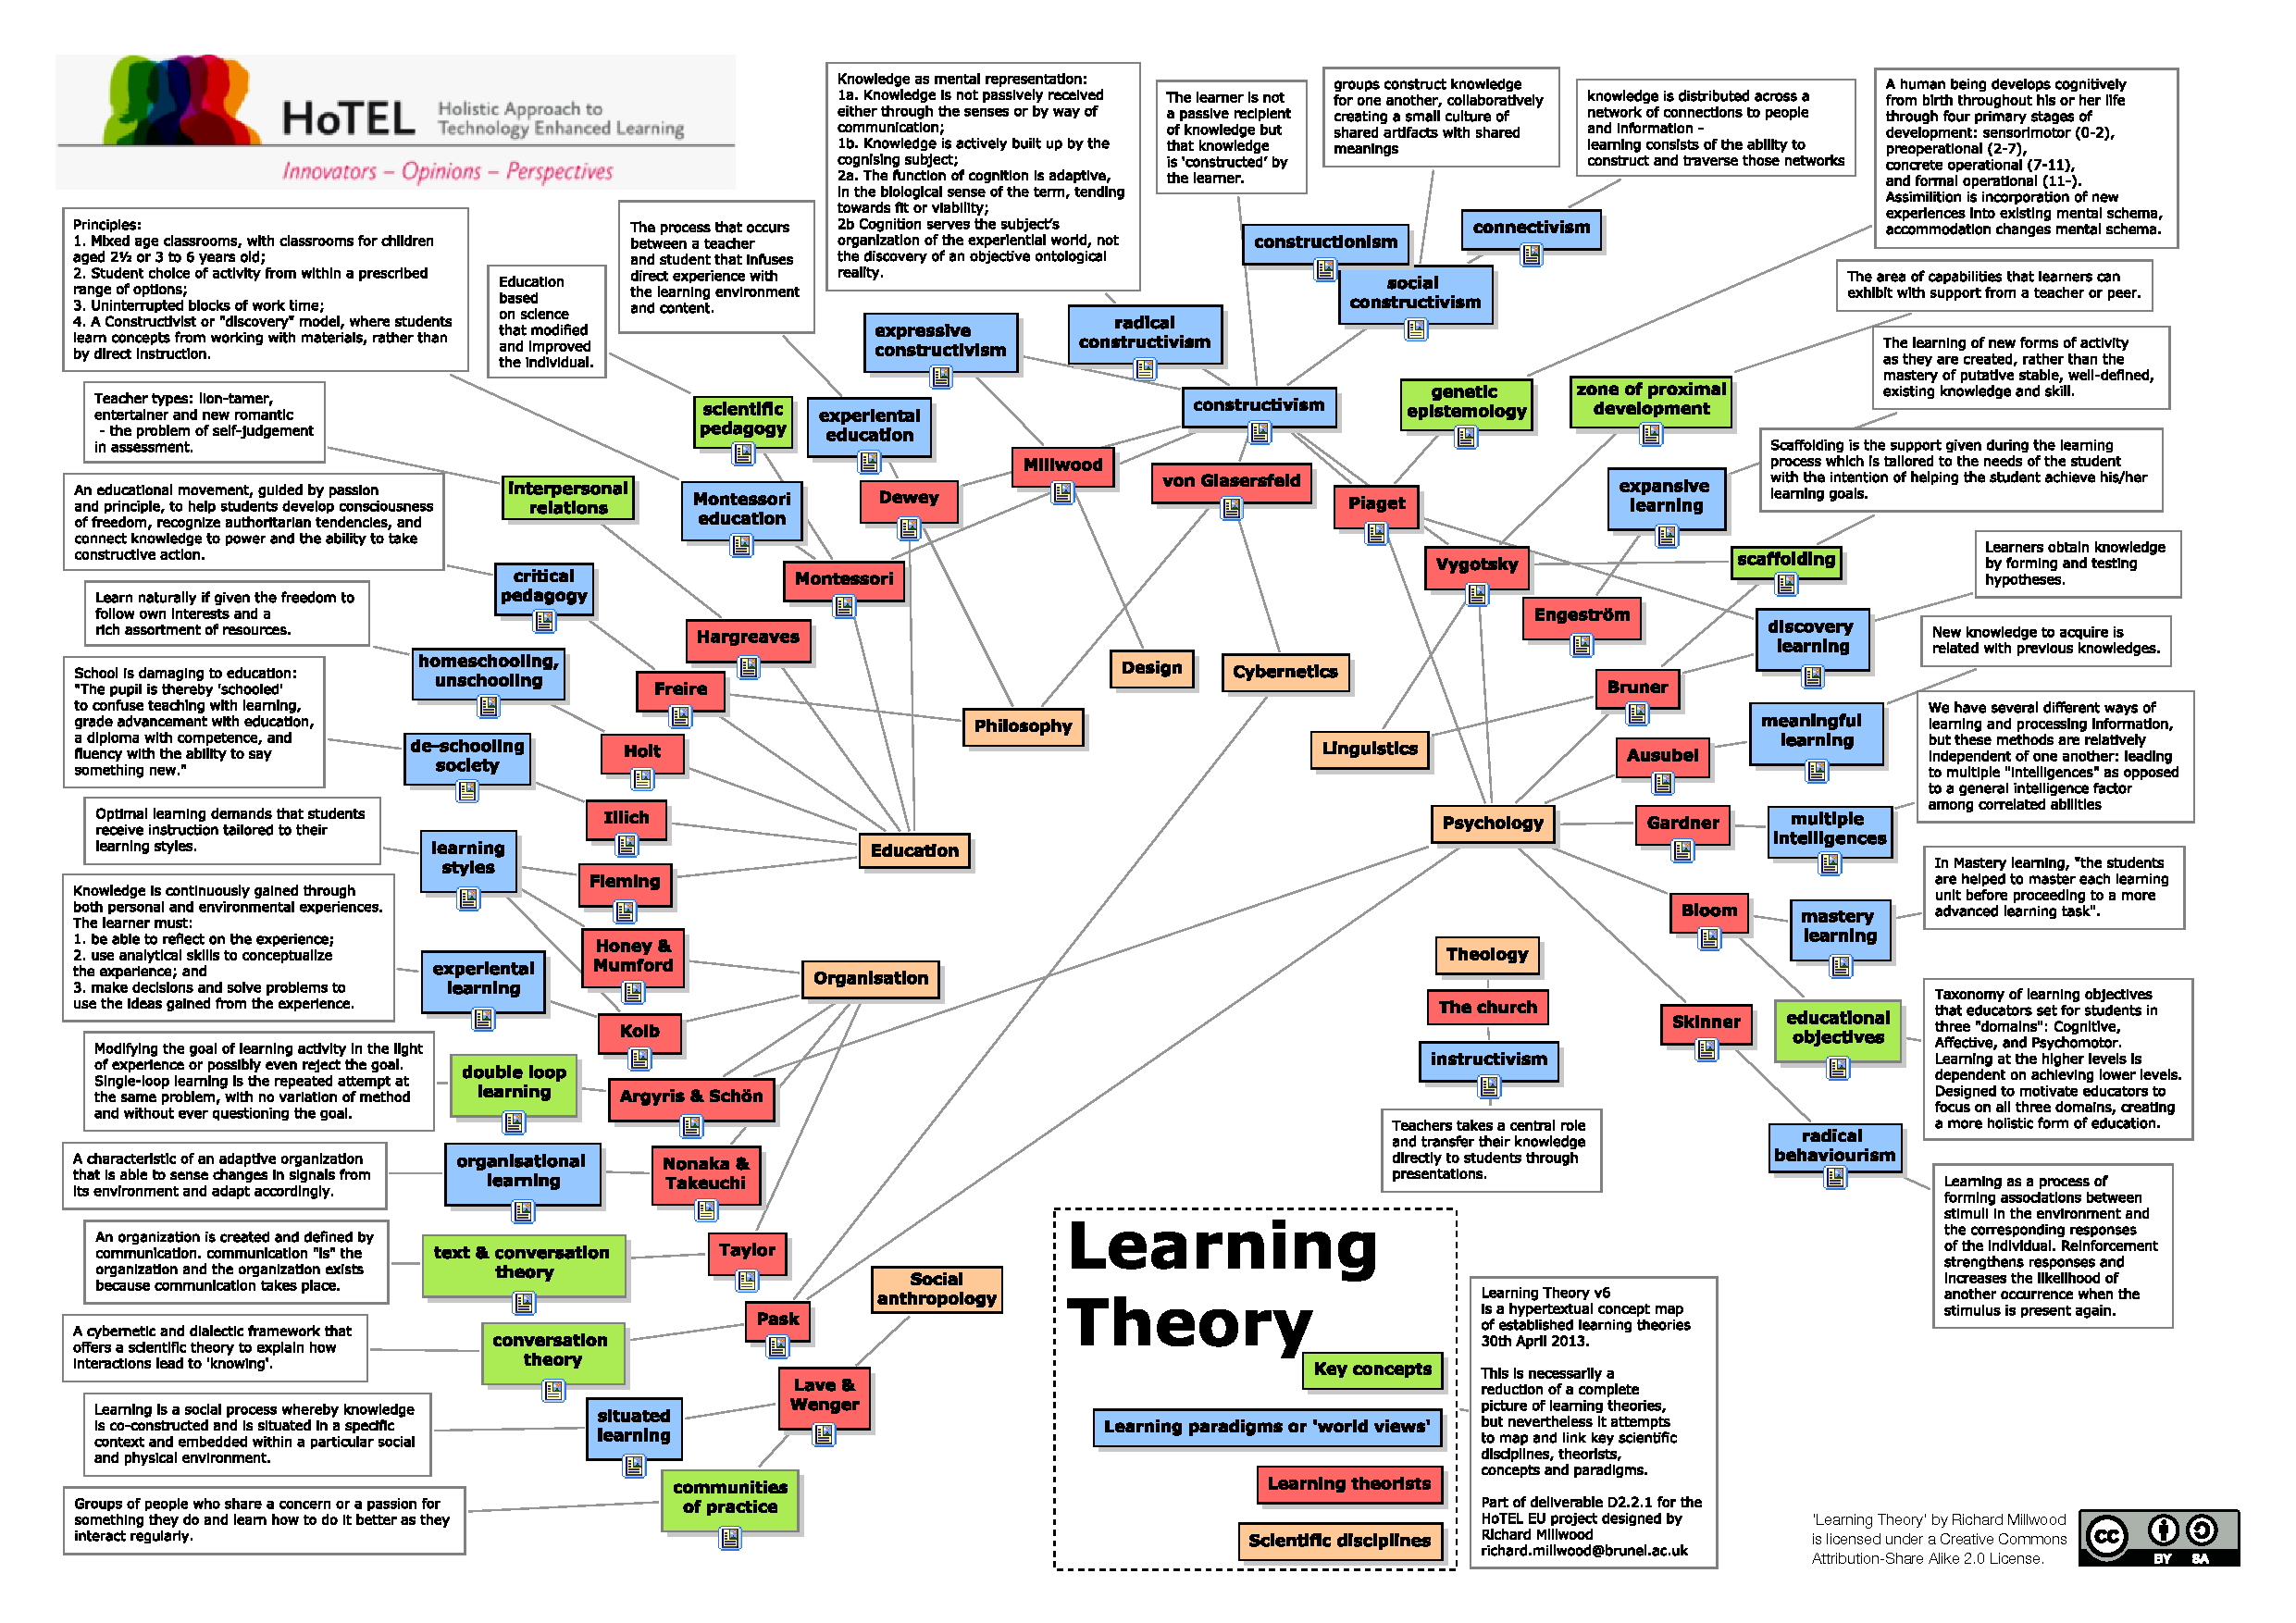
\includepdf[pages={-},fitpaper,rotateoversize]{assets/Learning-Theory.pdf}
